% Chapter 7: Artificial Neural Networks
\chapter{Artificial Neural Networks}\label{sec:ch07-ann}\label{chap:7}

A response surface model is a low-order polynomial. It works very well when the response is smooth over the
region studied, but it cannot follow sharp optima, saturation, plateaus or strong interactions of more than two
factors. An artificial neural network (ANN) is a flexible nonlinear regression model that can follow such
patterns, provided there are enough runs to estimate it and to check it on data it has not seen. The
\ui{ANN} page (navigation group \ui{Analysis}, page title \ui{Artificial Neural Network}) fits multilayer
perceptrons to the continuous responses of the project and answers four questions:
\begin{enumerate}
  \item Are the data adequate for an ANN at all (\ui{Data Adequacy})?
  \item Which network size is supported by the data (check~A, the cross-validated architecture search)?
  \item Does the fitted network generalize, or does it underfit or overfit (\ui{Fit Diagnosis})?
  \item Would more runs still improve the network, and roughly how many (check~B, the learning curve)?
\end{enumerate}
A network trained here can replace the RSM model of the same response in the model graphs, in the desirability and
NSGA optimizations, in the sensitivity study and on the \ui{Prediction \& Confirmation} page
(Section~\ref{sec:ch07-use}). Binomial and Poisson responses are not modeled with an ANN; they are analyzed with
logistic or Poisson regression on the \ui{RSM Analysis} page.

The examples in this chapter use the case study \ui{Dye Adsorption (ANN, 40 runs)} (\menupath{File $\rightarrow$
Case Studies\dots}). It contains 40 historical runs placed by a Latin hypercube in four factors (A: pH 2--10,
B: Adsorbent Dose 0.5--4~g/L, C: Contact Time 10--120~min, D: Initial Concentration 20--200~mg/L) and one
response, R1: Removal Efficiency (\%), which ranges from 2.73 to 58.45~\%. The response has a pH optimum, a
kinetic and an isotherm effect, so it is strongly nonlinear. All numbers below were obtained with the default
settings, random seed 1 and one CPU core; the screenshots show the same state.

\section{Layout of the page and suggested workflow}\label{sec:ch07-layout}

The page has a scrollable control panel on the left and ten result tabs on the right
(Figure~\ref{fig:ch07-summary}). At the top of the left panel, \ui{Show response:} selects the response whose
results are shown. Changing it re-runs the data adequacy assessment and refreshes all tabs. Below it are four
groups:
\begin{itemize}
  \item \ui{1. Data Adequacy}: the verdict, the buttons \ui{Assess Data Adequacy} and
    \ui{Learning Curve (Enough Data?)} (check~B).
  \item \ui{2. ANN Model}: one network per response or one network for several responses.
  \item \ui{3. Network Settings}: algorithm, normalization, activation, early stopping, network size, data
    split, restarts, epochs, seed, CPU cores and the button \ui{Train ANN (This Response)}.
  \item \ui{4. Optimize Layers \& Neurons (Automatic)}: the settings of the architecture search (check~A) and the
    buttons \ui{Search Architecture (This Response)} and \ui{Optimize All Responses (One Click)}.
\end{itemize}
Under the groups are a status line, the check box \ui{Use this response's ANN for graphs, optimization, NSGA-II \&
prediction} and a reminder of the suggested workflow:
\begin{enumerate}
  \item Fit the RSM model of the response first on the \ui{RSM Analysis} page. The ANN page uses the current RSM
    model as the reference in every comparison.
  \item Read the \ui{Data Adequacy} report (it is produced automatically when the page opens).
  \item Click \ui{Optimize All Responses (One Click)} or \ui{Search Architecture (This Response)}. The application
    chooses the number of hidden layers and neurons by cross-validation and trains the final network.
  \item Read the \ui{Fit Diagnosis} on the \ui{Summary \& Diagnosis} tab and compare with RSM on the
    \ui{Architecture Search} tab.
  \item If the data are borderline, run \ui{Learning Curve (Enough Data?)}.
  \item Tick \ui{Use this response's ANN for graphs, optimization, NSGA-II \& prediction} only if the ANN
    predicts new data better than the RSM model.
\end{enumerate}

Table~\ref{tab:ch07-tabs} lists the result tabs. While a model is missing, the plot tabs show ``No ANN model yet''
and the \ui{Summary \& Diagnosis} tab explains how to train one.

\begin{table}[htbp]
\centering
\caption{Result tabs of the ANN page.}\label{tab:ch07-tabs}
\begin{tabularx}{\linewidth}{@{}lX@{}}
\toprule
Tab & Content \\
\midrule
\ui{Data Adequacy} & Report of the eleven adequacy checks, verdict, recommendations; response histogram and check
  summary (Section~\ref{sec:ch07-adequacy}). \\
\ui{Learning Curve} & Check~B: test $R^2$ against the number of training runs, power-law fit, estimate of the runs
  needed (Section~\ref{sec:ch07-learning}). \\
\ui{Summary \& Diagnosis} & Architecture, algorithm, data split, fit diagnosis, performance table, RSM comparison,
  factor importance (Section~\ref{sec:ch07-diagnosis}). \\
\ui{Architecture Search} & Check~A: all candidate networks, best per depth, selected network, comparison with
  RSM on the same test data (Section~\ref{sec:ch07-search}). \\
\ui{Regression Plots} & Output against target for training, validation, test and all data. \\
\ui{Training Performance} & Error per epoch for training, validation and test data. \\
\ui{Factor Importance} & Relative importance of each factor by Garson's method. \\
\ui{RSM vs ANN} & Predicted against actual values and residuals per run for both models. \\
\ui{Network Diagram} & Nodes and connections, colored by the sign of the weight. \\
\ui{Weights \& Biases} & All weights, biases and normalization parameters. \\
\bottomrule
\end{tabularx}
\end{table}

\section{The network model}\label{sec:ch07-model}

\subsection{Structure}

REGEN uses a fully connected feed-forward network (multilayer perceptron) with $L \ge 1$ hidden layers of
$h_1,\dots,h_L$ neurons and a linear output layer with $n_\text{out}$ outputs. There is no upper limit on the
number of layers or neurons. With the normalized input vector $\mathbf{x}_n$,
\begin{align}
  \mathbf{h}^{(0)} &= \mathbf{x}_n, \label{eq:ch07-input}\\
  \mathbf{h}^{(l)} &= f\!\left(\mathbf{W}^{(l)}\mathbf{h}^{(l-1)} + \mathbf{b}^{(l)}\right),
     \qquad l = 1,\dots,L, \label{eq:ch07-hidden}\\
  \mathbf{y}_n &= \mathbf{W}_\text{out}\,\mathbf{h}^{(L)} + \mathbf{b}_\text{out}, \label{eq:ch07-output}
\end{align}
where $\mathbf{W}^{(l)}$ ($h_l \times h_{l-1}$) and $\mathbf{b}^{(l)}$ are the weights and biases of layer $l$ and
$\mathbf{y}_n$ is the normalized output. The activation function of the hidden neurons is selected with
\ui{Activation function:}:
\begin{equation}
  \text{tansig: } f(a) = \tanh a, \qquad \text{logsig: } f(a) = \frac{1}{1+e^{-a}}. \label{eq:ch07-act}
\end{equation}
The default and recommended choice is \ui{tansig (tanh)}, which is centered on zero and matches the input range
$[-1,1]$ of the default normalization. The output layer is always linear, so the network can predict any value
of the response and is not limited to the range of the activation function.

The number of adjustable parameters (weights and biases) is
\begin{equation}
  W = \sum_{l=1}^{L} h_l\,(h_{l-1}+1) + n_\text{out}\,(h_L+1), \qquad h_0 = n_\text{in}.
  \label{eq:ch07-nweights}
\end{equation}
The network is written as the string $n_\text{in}$-$h_1$-$\cdots$-$h_L$-$n_\text{out}$. For the dye case
with one hidden layer of 3 neurons, the network is 4-3-1 with $W = 3\cdot 5 + 1\cdot 4 = 19$ weights. Below the
entry \ui{Neurons per hidden layer:} the page shows the number of layers and of weights for the current entry,
for example ``1 hidden layer, 19 weights''.

\subsection{Inputs, outputs and normalization}\label{sec:ch07-norm}

The network inputs are the factors in coded units: $-1$ to $+1$ for process factors and pseudo-components for
mixture components. A categorical factor with $m$ levels becomes $m$ one-hot input columns (one column per level,
1 for the level of the run and 0 otherwise), so $n_\text{in}$ counts these columns. The responses enter in their
original units. The response transformation chosen on the \ui{RSM Analysis} page is \emph{not} used by the ANN.

Before training, every input column and every output is normalized by
\begin{equation}
  x_n = \text{base} + \frac{x - \text{offset}}{\text{scale}}, \qquad
  y = (y_n - \text{base})\cdot\text{scale} + \text{offset}, \label{eq:ch07-normalize}
\end{equation}
where the second relation converts the network output back to response units. The parameters depend on the option
\ui{Normalization:} (Table~\ref{tab:ch07-norm}). They are computed from the \emph{training and validation} runs
only; the test runs never influence them, so no information leaks from the test data into the model. A scale of
zero (a constant column) is replaced by 1. A response that is constant over the training and validation runs
cannot be modeled (message ``Constant response - the ANN cannot be trained.'').

\begin{table}[htbp]
\centering
\caption{Normalization options (\ui{Normalization:}); min, max, mean and SD are computed per column over the
training and validation runs.}\label{tab:ch07-norm}
\begin{tabularx}{\linewidth}{@{}Xllll@{}}
\toprule
Option & offset & scale & base & Range of $x_n$ \\
\midrule
\ui{Min-max to [-1, 1] (mapminmax) - recommended} (default) & min & (max $-$ min)/2 & $-1$ & $[-1,1]$ \\
\ui{Min-max to [0, 1]} & min & max $-$ min & 0 & $[0,1]$ \\
\ui{Z-score standardization (mapstd): mean 0, SD 1} & mean & SD & 0 & mean 0, SD 1 \\
\ui{No normalization (for comparison)} & 0 & 1 & 0 & unchanged \\
\bottomrule
\end{tabularx}
\end{table}

Normalization matters because the inputs and outputs have very different ranges. In the dye case the largest
range (Initial Concentration, 180~mg/L) is 51 times the smallest (Adsorbent Dose, 3.5~g/L). Without normalization
the large variables dominate the error and the gradients, and the tanh neurons saturate. The option \ui{No
normalization (for comparison)} exists only to demonstrate this. The same transformations can be inspected on
the \ui{Data Normalization} page (navigation group \ui{Tools}).

\subsection{Separate and combined networks}\label{sec:ch07-combined}

Group \ui{2. ANN Model} offers two options:
\begin{itemize}
  \item \ui{Separate - one network per response} (default): each response gets its own network and its own
    architecture. This is usually more accurate.
  \item \ui{Combined - one network for several responses}: one multi-output network models all responses checked
    in the list \ui{Responses combined in one network:}. Non-continuous responses are listed with the suffix
    ``(not continuous)'' and cannot be checked; at least two continuous responses are needed. The buttons change
    to \ui{Train Combined ANN} and \ui{Search Architecture (Combined Model)}, and \ui{Optimize All Responses (One
    Click)} is hidden.
\end{itemize}
In a combined network the hidden layers are shared and the output layer has one linear neuron per response. The
training error sums over all outputs, the normalized errors are averaged over the outputs, and the plots of a
response show its own output. A combined model is more compact and can be useful when the responses are
physically related, but every response then has to accept the same hidden layers. Training a new network for a
response that belongs to a combined network breaks the old combined network apart.

\section{Network settings and training}\label{sec:ch07-training}

\subsection{How to train a network by hand}

\begin{enumerate}
  \item Select the response in \ui{Show response:}.
  \item In \ui{3. Network Settings}, choose the algorithm, normalization and activation, and type the neurons per
    hidden layer, for example \texttt{5} (one layer), \texttt{8, 4} (two layers) or \texttt{64, 32, 16, 8}.
    Commas, semicolons or spaces separate the layers.
  \item Check the data split and the other settings (Table~\ref{tab:ch07-settings}).
  \item Click \ui{Train ANN (This Response)}. The progress line shows ``Training \dots: restart $i$/$n$'' and the
    \ui{Stop} button interrupts the work. When training is finished the status line reads, for example, ``Done:
    4-3-1, Overfitting'' and the \ui{Summary \& Diagnosis} tab opens.
\end{enumerate}
Setting the network size by hand is useful for teaching and for comparisons. For a model that will be used,
let the architecture search choose the size (Section~\ref{sec:ch07-search}).

\begin{table}[htbp]
\centering
\caption{Options of group \ui{3. Network Settings}.}\label{tab:ch07-settings}
\begin{tabularx}{\linewidth}{@{}>{\raggedright\arraybackslash}p{3.3cm}>{\raggedright\arraybackslash}p{3.2cm}>{\raggedright\arraybackslash}p{2.15cm}X@{}}
\toprule
Option & Values & Default & Meaning \\
\midrule
\ui{Algorithm:} & \ui{Bayesian Regularization (trainbr)}, \ui{Levenberg-Marquardt (trainlm)}, \ui{Adam mini-batch}
  & trainbr & Training algorithm (Section~\ref{sec:ch07-algorithms}). \\
\ui{Normalization:} & four options & mapminmax & Table~\ref{tab:ch07-norm}. \\
\ui{Activation function:} & \ui{tansig (tanh)}, \ui{logsig (sigmoid)} & tansig & Hidden-layer activation,
  Eq.~\eqref{eq:ch07-act}. \\
\ui{Early stopping (use validation data)} & on/off & on & Stop when the validation error no longer improves and
  keep the best weights. \\
\ui{Max validation failures:} & 1--100 & 6 & Number of epochs without validation improvement before training
  stops (shown only with early stopping). \\
\ui{Neurons per hidden layer:} & list of integers & \texttt{5} & One number per hidden layer; no limit. \\
\ui{Training data:}, \ui{Validation data:}, \ui{Test data:} & 0--100~\% each, sum 100~\% & 70/15/15 (85/0/15
  without early stopping) & Random data split. Reset to the default whenever the algorithm or the early-stopping
  box changes. \\
\ui{Restarts (initializations):} & 1--100 & 10 & Independent random initializations; the best is kept. \\
\ui{Maximum epochs:} & 10--5000 & 500 & Upper limit on training iterations. \\
\ui{Random seed:} & 0--999999 & 1 & Fixes the data split and the initial weights. \\
\ui{CPU cores (parallel):} & 1 to the number of logical CPUs & all but one & Section~\ref{sec:ch07-parallel}. \\
\bottomrule
\end{tabularx}
\end{table}

The page refuses inconsistent settings with a message: ``Training + validation + test percentages must add up to
100\%.'', ``Early stopping requires validation data (> 0\%).'', ``Enter the neurons per hidden layer as numbers
separated by commas. Example: 20, 10, 5'' or ``At least 1 hidden layer is required, and each layer needs at least
1 neuron.''. At least 4 complete runs are needed (``Too little data to train an ANN (at least 4 complete runs
required).''), and at least 2 training runs. Only runs in which all factors and the response are present are
used; runs excluded on the \ui{Data} page count as empty.

\subsection{Data split and early stopping}\label{sec:ch07-split}

For $n$ complete runs and the fractions $(p_\text{tr}, p_\text{va}, p_\text{te})$, the runs are randomly permuted
(the permutation depends only on \ui{Random seed:}) and
\begin{equation}
  n_\text{va} = \operatorname{round}(n\,p_\text{va}),\qquad n_\text{te} = \operatorname{round}(n\,p_\text{te}),
  \qquad n_\text{tr} = n - n_\text{va} - n_\text{te}, \label{eq:ch07-split}
\end{equation}
where $n_\text{va}$ and $n_\text{te}$ are raised to 1 when their fraction is positive and $n \ge 6$. The three
sets have distinct roles:
\begin{itemize}
  \item \emph{training} runs determine the weights;
  \item \emph{validation} runs are watched during training and stop it when the network starts to fit noise
    (early stopping); they also take part in choosing the best restart;
  \item \emph{test} runs are never used during training. They give an independent estimate of the prediction
    error on new data.
\end{itemize}
With 40 runs and 70/15/15~\%, the dye case uses 28 training, 6 validation and 6 test runs.

Early stopping \citep{prechelt1998}: at every epoch the validation error is computed before the weights are
updated. If it is lower than the best value so far, the weights are stored and the failure counter is reset;
otherwise the counter is increased. Training stops when the counter reaches \ui{Max validation failures:}, and the
stored weights (lowest validation error) are used. If early stopping is switched off, the validation runs are
merged into the training set.

\subsection{Weight initialization and restarts}

The initial weights of each hidden layer follow \citet{nguyen1990}. For a layer with $n_i$ inputs and $n_o$
neurons,
\begin{equation}
  \beta_\text{NW} = 0.7\,n_o^{1/n_i}, \qquad
  \mathbf{w}_k \sim U(-1,1)^{n_i} \text{ rescaled to } \|\mathbf{w}_k\| = \beta_\text{NW}, \qquad
  b_k \sim U(-\beta_\text{NW}, \beta_\text{NW}), \label{eq:ch07-nw}
\end{equation}
where $\mathbf{w}_k$ is the weight vector of neuron $k$. This spreads the active regions of the neurons over the
input range. The output weights and biases start from $U(-0.5, 0.5)$.

Training a network is a nonconvex problem: different starting weights can end in different local minima. REGEN
therefore trains \ui{Restarts (initializations):} networks from independent random starts (restart $r$ uses its
own random generator derived from the seed and $r$) and keeps the restart with the lowest score
\begin{equation}
  S = \tfrac{1}{2}\left[\text{MSE}_\text{tr}(\mathbf{w}^*) + \text{MSE}_\text{va}(\mathbf{w}^*)\right]
  \quad\text{(with validation data)}, \qquad S = \text{MSE}_\text{tr}(\mathbf{w}^*) \quad\text{(without)},
  \label{eq:ch07-score}
\end{equation}
computed on the normalized scale for the weights $\mathbf{w}^*$ that are kept. The test runs take no part in the
choice. Because each restart has its own generator, the result is the same whether the restarts run one after
the other or in parallel.

\subsection{Training algorithms}\label{sec:ch07-algorithms}

Let $\mathbf{e} = \mathbf{y}_n - \hat{\mathbf{y}}_n$ be the vector of errors of all training runs and outputs on
the normalized scale, $\mathbf{w}$ the vector of all $W$ weights and $\mathbf{J} = \partial\hat{\mathbf{y}}_n /
\partial\mathbf{w}$ the Jacobian, computed exactly by backpropagation.

\paragraph{Levenberg-Marquardt (trainlm).} Each epoch solves \citep{hagan1994}
\begin{equation}
  \Delta\mathbf{w} = \left(\mathbf{J}^\top\mathbf{J} + \mu\mathbf{I}\right)^{-1}\mathbf{J}^\top\mathbf{e},
  \label{eq:ch07-lm}
\end{equation}
starting from $\mu = 10^{-3}$. A step that lowers the training sum of squares is accepted and $\mu$ is divided by
10; otherwise $\mu$ is multiplied by 10 and the step is recomputed. Small $\mu$ gives a Gauss-Newton step, large
$\mu$ a short gradient-descent step. Training ends at \ui{Maximum epochs:} (``Maximum epochs''), when the largest
gradient component $|\mathbf{J}^\top\mathbf{e}|$ falls below $10^{-7}$ (``Minimum gradient''), when $\mu$ exceeds
$10^{10}$ (``Maximum μ''), by early stopping (``Early stopping (no validation improvement 6×)'') or by the
\ui{Stop} button (``Stopped by user'').

\paragraph{Bayesian regularization (trainbr).} This is the default and the recommended algorithm for the small
data sets typical of designed experiments. It minimizes \citep{mackay1992,foresee1997}
\begin{equation}
  F(\mathbf{w}) = \beta E_D + \alpha E_W, \qquad E_D = \sum_i e_i^2, \qquad E_W = \sum_k w_k^2,
  \label{eq:ch07-br}
\end{equation}
so large weights are penalized and the network stays smooth. The Levenberg-Marquardt step on $F$ is
\begin{equation}
  \Delta\mathbf{w} = \left(\beta\mathbf{J}^\top\mathbf{J} + (\mu+\alpha)\mathbf{I}\right)^{-1}
  \left(\beta\mathbf{J}^\top\mathbf{e} - \alpha\mathbf{w}\right), \label{eq:ch07-brstep}
\end{equation}
with $\mu = 5\times10^{-3}$ at the start and the same rules for $\mu$ and the same stop criteria as trainlm. The
hyperparameters start at $\alpha = 0.01$ and $\beta = 1$ and are kept fixed during a warm-up of 15 epochs, so the
network can learn the main pattern before the regularization is tuned. From epoch 15 on, after every accepted
step, the evidence framework updates them with the Gauss-Newton approximation of the Hessian:
\begin{align}
  \gamma &= W - \alpha\,\operatorname{tr}\!\left[\left(\beta\mathbf{J}^\top\mathbf{J} + \alpha\mathbf{I}\right)^{-1}
  \right], \qquad \gamma \leftarrow \min\!\left(\max(\gamma, 1),\, N-1\right), \label{eq:ch07-gamma}\\
  \alpha &= \frac{\gamma}{2E_W}, \qquad \beta = \frac{N-\gamma}{2E_D}, \qquad N = n_\text{tr}\,n_\text{out}.
  \label{eq:ch07-alphabeta}
\end{align}
The quantity $\gamma$ is the effective number of parameters: the number of weights that the data actually
determine. It is reported on the \ui{Summary \& Diagnosis} tab as ``effective parameters $\gamma$ = \dots{} of
$W$''. A value much smaller than $W$ means that the regularization has switched off part of the network.

With early stopping, trainbr records the best validation error at every epoch but counts validation failures
only after the warm-up, so training always runs at least 15 + \ui{Max validation failures:} epochs. The weights
and the $\gamma$ of the best validation epoch are used. If that epoch lies inside the warm-up, $\gamma$ has not
yet been estimated (it still has its starting value $W$), and the summary says so instead of giving a number:
``effective parameters $\gamma$ not estimated yet (best epoch $N$ lies within the warm-up; $\gamma$ is first
estimated after epoch 15)''. In that case the regularization acted only through the small fixed $\alpha$. Without early stopping, the final weights are used. In the architecture search and the learning curve
(but not in \ui{Train ANN}) training also stops with ``Converged'' when the training error changed by less than a
relative $10^{-5}$ over the last 10 epochs.

\paragraph{Adam (mini-batch).} Levenberg-Marquardt and Bayesian regularization need a $W\times W$ matrix and a
Jacobian with $n_\text{tr}\,n_\text{out}\,W$ elements. When $W > 2000$ or $n_\text{tr}\,n_\text{out}\,W > 3\times
10^{7}$, REGEN therefore switches automatically to Adam \citep{kingma2015}; the entry below \ui{Neurons per
hidden layer:} warns ``(large: trained automatically with Adam)'' and the summary adds ``(selected automatically:
network too large for Levenberg-Marquardt)''. Adam can also be chosen directly. It minimizes the mean squared
error with mini-batches of $\min(256, \max(16, \lfloor n_\text{tr}/20\rfloor))$ runs, reshuffled every epoch:
\begin{equation}
  \mathbf{m} \leftarrow 0.9\,\mathbf{m} + 0.1\,\mathbf{g}, \qquad
  \mathbf{v} \leftarrow 0.999\,\mathbf{v} + 0.001\,\mathbf{g}^2, \qquad
  \mathbf{w} \leftarrow \mathbf{w} - \eta\,\frac{\hat{\mathbf{m}}}{\sqrt{\hat{\mathbf{v}}} + 10^{-8}},
  \label{eq:ch07-adam}
\end{equation}
where $\mathbf{g}$ is the gradient, $\hat{\mathbf{m}}$ and $\hat{\mathbf{v}}$ are the bias-corrected moments and
$\eta$ starts at $2\times10^{-3}$. The monitored error is the validation error (or the training error without
validation data). It must improve by a relative $10^{-4}$; after 8 epochs without improvement $\eta$ is halved,
and training stops after $\max(\text{\ui{Max validation failures:}}, 20)$ epochs without improvement. Adam is
meant for very large networks or data sets; for designed experiments with tens of runs use trainbr.

\subsection{Error measures}\label{sec:ch07-metrics}

For each set (training, validation, test, all) the \ui{Performance} table reports, in response units,
\begin{equation}
\begin{gathered}
  R^2 = 1 - \frac{\sum (y_i - \hat y_i)^2}{\sum (y_i - \bar y)^2}, \qquad
  \text{RMSE} = \sqrt{\tfrac{1}{n}\textstyle\sum (y_i-\hat y_i)^2}, \\
  \text{MAE} = \tfrac{1}{n}\textstyle\sum |y_i-\hat y_i|, \qquad
  \text{AAD} = \tfrac{100}{n}\textstyle\sum \frac{|y_i-\hat y_i|}{|y_i|},
\end{gathered}\label{eq:ch07-metrics}
\end{equation}
and $R$, the Pearson correlation between target and output. $R^2$ of a set is computed with the mean of that set,
so a small test set with a narrow spread can give a low or negative $R^2$ even when the errors are small. AAD is
not defined if a response value is zero.

The diagnosis uses the \emph{normalized mean squared error}
\begin{equation}
  \text{NMSE}_\text{set} = \frac{1}{n_\text{out}}\sum_{k=1}^{n_\text{out}}
  \frac{\text{MSE}_{k,\text{set}}}{\operatorname{var}(y_k)}, \label{eq:ch07-nmse}
\end{equation}
where $\operatorname{var}(y_k)$ is the variance of response $k$ over all runs used. NMSE $=0$ is a perfect fit and
NMSE $=1$ is no better than predicting the mean; $1-\text{NMSE}$ is an $R^2$ on a common scale for all sets.

\subsection{Fit diagnosis of a single split}\label{sec:ch07-diagnose}

After training, the network is classified from the training error $E_\text{tr}$ and the error on new data
$E_\text{gen}$, the mean of the validation and test NMSE. If the data contain replicated runs (runs with identical
factor settings), the measurement noise is expressed on the same scale,
\begin{equation}
  \nu = \frac{s_\text{pe}^2}{\operatorname{var}(y)}, \label{eq:ch07-noise}
\end{equation}
where $s_\text{pe}$ is the pure-error standard deviation of the replicates (averaged over the outputs of a combined
network). The rules are applied in this order:
\begin{enumerate}
  \item Noise rule (only with replicates): $E_\text{tr} < 0.5\,\nu$ gives \ui{Overfitting} (``training error is
    below the measurement noise - the network is memorizing noise'').
  \item $E_\text{gen} > 2E_\text{tr}$ and $E_\text{gen} - E_\text{tr} > 0.02$ gives \ui{Overfitting} (``error on
    new data is \dots{}× the training error'').
  \item $E_\text{tr} > \ell$ and $E_\text{gen} < 1.5E_\text{tr} + 0.02$ gives \ui{Underfitting} (``training $R^2$
    is only \dots{} and the error on new data is similar - network capacity is too low''), with $\ell = \max(3\nu,
    0.1)$ when the noise is known and $\ell = 0.2$ otherwise.
  \item Otherwise the status is \ui{Good fit}.
\end{enumerate}
Without validation and test runs the status is \ui{Underfitting} if $E_\text{tr} > 0.2$ and \ui{Cannot be
assessed yet} otherwise. The noise rule needs replicates: without them the pure error is unknown and the report
says that the rule was not used. In the BBD extraction case of Chapter~\ref{chap:5}, the five center points give $s_\text{pe}
= 0.340$ for Yield, so $\nu = 0.340^2/25.92 = 0.0045$ and a training NMSE below 0.0022 would be flagged as
memorizing noise. The dye case has no replicates, so the rule is inactive there.

A single split of a small data set is a weak basis for this decision: with 40 runs and 15~\% test data, the test
error rests on 6 runs. The architecture search therefore provides a cross-validated diagnosis, which takes
precedence (Section~\ref{sec:ch07-diagnosis}).

\section{Data adequacy}\label{sec:ch07-adequacy}

\paragraph{Purpose.} Before a network is trained, the \ui{Data Adequacy} report checks whether the data can
support an ANN and can test it honestly: enough runs for the number of weights, enough levels to learn curvature,
a reasonable signal-to-noise ratio, no extreme outliers, and a factor space without large gaps.

\paragraph{How to use.} The assessment runs automatically when the page opens or the response changes; click
\ui{Assess Data Adequacy} to repeat it (for example after excluding runs). The verdict also appears in group
\ui{1. Data Adequacy}, colored green, amber or red. The training fraction used by the checks is the sum of the
training and validation percentages (at least 50~\%), so $n_\text{train} = \lfloor 0.85\,N\rfloor$ with the
default split.

\paragraph{Checks.} Table~\ref{tab:ch07-adequacy} lists the checks and their thresholds. A binomial or Poisson
response stops the assessment at once (``Not adequate - the response is not continuous''), as does a response with
fewer than 3 complete runs.

\begin{table}[htbp]
\centering
\small
\caption{Checks of the \ui{Data Adequacy} report. $N$ = complete runs, $W_2$ = weights of an
$n_\text{in}$-2-1 network.}\label{tab:ch07-adequacy}
\begin{tabularx}{\linewidth}{@{}>{\raggedright\arraybackslash}p{3.7cm}>{\raggedright\arraybackslash}X>{\raggedright\arraybackslash}p{4.1cm}@{}}
\toprule
Check & Value and meaning & Status \\
\midrule
\ui{Complete data} & Number of complete runs. & Good $N\ge30$; Caution $12\le N<30$; Not adequate $N<12$ \\
\ui{Training rows / weights ratio} & $n_\text{train}/W_2$; also the largest single hidden layer with
  $W\le n_\text{train}$ (trainlm) and $W\le 2n_\text{train}$ (trainbr). & Good $\ge3$; Caution $\ge1$; Not adequate
  $<1$ \\
\ui{Factor levels} & Distinct levels of each numeric factor. & Caution if a factor has fewer than 3 levels (no
  curvature can be learned) \\
\ui{Data per level of} \dots & Runs per level of a categorical factor. & Good $\ge5$; Caution $\ge2$; Not adequate
  $<2$ \\
\ui{Signal / noise ratio} & $\text{SD}(y)/s_\text{pe}$ from replicated runs. & Good $\ge4$; Caution $\ge2$; Not
  adequate $<2$; Info ``cannot be calculated'' without replicates \\
\ui{Response outliers (|robust z| > 3.5)} & Runs with $|0.6745\,(y-\tilde y)/\text{MAD}| > 3.5$ ($\tilde y$ =
  median). & Caution if any \\
\ui{Response distribution} & Skewness and max/min. & Caution if $|\text{skewness}|>1$ or max/min $>10$ \\
\ui{Factor correlation} & Largest $|r|$ between two numeric factors (not for mixtures). & Good $<0.5$; Caution
  $<0.9$; Not adequate $\ge0.9$ \\
\ui{Factor space coverage} & Largest distance from 3000 random points in the coded factor space to the nearest run,
  divided by $\sqrt{k}$ (not for mixtures). & Good if $\le0.35$ and every factor spans $\ge90$~\% of its range;
  else Caution \\
\ui{Need for a nonlinear model} & RSM Predicted $R^2$ and lack-of-fit $p$ (OLS analysis only). & Good if lack of
  fit $p<0.05$; Info otherwise (with a note if Pred $R^2\ge0.95$) \\
\ui{Variable range differences} & Largest/smallest range of factors and response. & Info (note if $>100$) \\
\bottomrule
\end{tabularx}
\end{table}

\paragraph{Verdict and recommendations.} Any \ui{Not adequate} check gives ``Not adequate for ANN (fix or add
data first)''; three or more cautions give ``Adequate with many caveats - ANN results need strict validation'';
one or two cautions give ``Adequate with caveats''; otherwise ``Adequate for ANN modeling''. The
\ui{Recommendations} list the algorithm (trainbr, especially with fewer than 50 runs), the data split (the
default 70/15/15~\% with early stopping, judged by cross-validation when there are fewer than 30 runs), a size for
a network set by hand (the weights kept below twice the training runs), a realistic RMSE target equal to the
noise when replicates exist, a note for skewed responses (see below), and ``Add runs (e.g. Augment Design on the
Data page) before relying on the ANN.'' when a check failed or $N<12$. The note under the table recalls the rule
of thumb for networks set by hand (weights $\le$ training runs, or $\le 2\times$ with trainbr) and that the
architecture search has no weight limit by default. Below the report, a histogram of the response (with a band of
$\pm$ the noise around the mean when replicates exist) and a bar chart count the statuses.

\paragraph{What to do when checks fail.} Too few runs or a ratio below 1: add runs, or stay with RSM. Factors
with two levels: the ANN cannot learn curvature in them, so it offers nothing over an interaction model. Low
signal-to-noise: no model will be accurate; improve the measurement or replicate. Outliers: check the records
before training, since a network will try to follow them. Correlated factors (common in historical data): effects
cannot be separated and the factor importance is unreliable. Coverage gaps: predictions inside the gaps are
extrapolations; the \ui{Data Readiness} page can suggest space-filling runs.

\paragraph{Example.} For the dye case the verdict is ``Adequate with caveats'' (Figure~\ref{fig:ch07-adequacy}):
\ui{Complete data} 40 runs (Good); \ui{Training rows / weights ratio} ``2.62 (4-2-1 network, 13 weights)''
(Caution, $34/13$); factor levels 40, 39, 40, 40 (Good); signal/noise ``cannot be calculated'' (no replicates);
no outliers; \ui{Response distribution} ``skewness 0.85, max/min 21.4'' (Caution); factor correlation 0.25 (A--C,
Good); coverage gap 0.29 (Good); RSM Pred $R^2$ 0.5620 (Info); range ratio 51.2 (Info). The recommendations
include ``1 hidden layer $\le$ 11 neurons or 2 hidden layers $\le$ 5 neurons per layer'' for a network set by
hand. The two cautions are mild; the data can support a small network.

\begin{figure}[htbp]
\centering
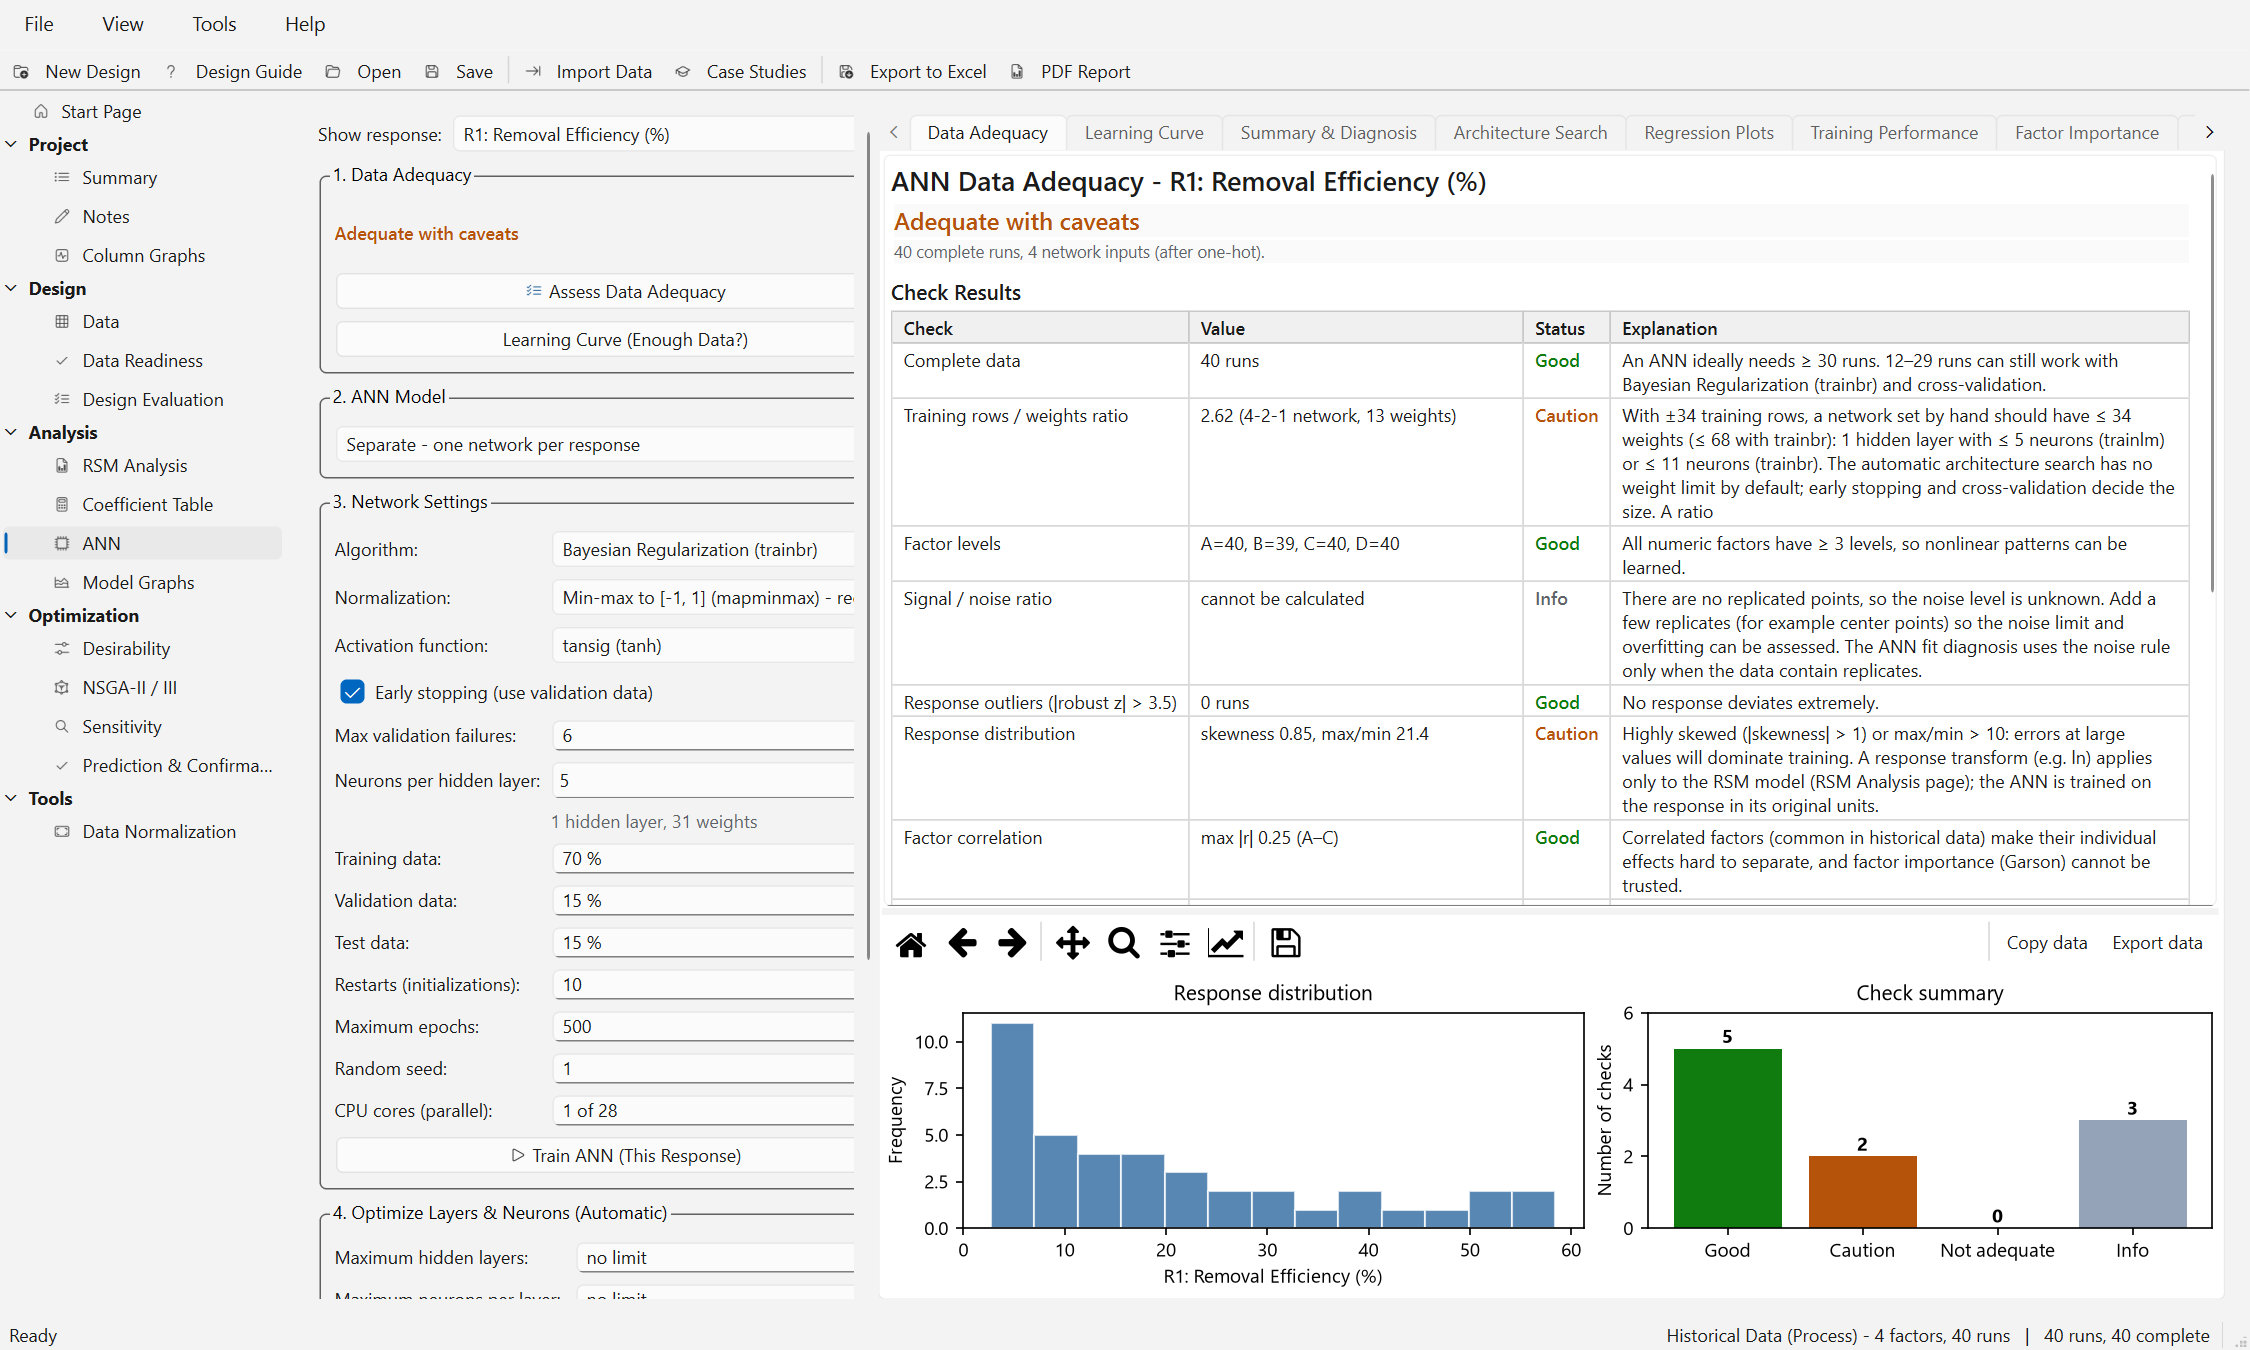
\includegraphics[width=\linewidth]{ann_adequacy.png}
\caption{\ui{Data Adequacy} tab for the dye adsorption case: verdict ``Adequate with caveats'', the table of
checks, the response histogram and the summary of statuses (5 Good, 2 Caution, 3 Info).}
\label{fig:ch07-adequacy}
\end{figure}

\paragraph{Skewed responses.} When the \ui{Response distribution} check gives Caution, its explanation reads
``Highly skewed (|skewness| > 1) or max/min > 10: errors at large values will dominate training. A response
transform (e.g. ln) applies only to the RSM model (RSM Analysis page); the ANN is trained on the response in its
original units.'' The recommendation adds: ``Skewed response: a response transform (e.g. ln) on the RSM Analysis
page applies to the RSM model only. The ANN is trained on the response in its original units; the Normalization
options only rescale it linearly and do not reduce the skewness.'' The normalization maps the response to
$[-1,1]$, but large values continue to dominate the squared error, so judge the network also by its relative
errors (AAD) and by the residuals at small response values.

\section{Check A: cross-validated architecture search}\label{sec:ch07-search}

\paragraph{Purpose.} The number of hidden layers and neurons controls the flexibility of the network: too few
neurons underfit, too many fit the noise. The architecture search finds the smallest network that predicts new
data as well as any larger one, using cross-validation \citep{hastie2009} rather than a single random split.

\subsection{How to use}

\begin{enumerate}
  \item Set the algorithm, normalization, activation, \ui{Max validation failures:} and \ui{Random seed:} in
    \ui{3. Network Settings}. These settings are used for every candidate network.
  \item In \ui{4. Optimize Layers \& Neurons (Automatic)}, keep the defaults (Table~\ref{tab:ch07-search}) unless
    the computation is too long.
  \item Click \ui{Search Architecture (This Response)} for the shown response, or \ui{Optimize All Responses (One
    Click)} to search and train a network for every continuous response in turn. Tick \ui{When finished, use ANN
    for graphs/optimization} if the networks should immediately replace the RSM models.
  \item Follow the progress line, for example ``R1 - 2 hidden layers: architecture 3-3 (candidate 8)''. \ui{Stop}
    ends the search; the results so far are kept and marked as incomplete.
  \item When the search ends, the selected architecture is trained on all data with the \ui{Network Settings}
    (Section~\ref{sec:ch07-final}) and the \ui{Architecture Search} tab opens.
\end{enumerate}

\begin{table}[htbp]
\centering
\caption{Options of group \ui{4. Optimize Layers \& Neurons (Automatic)}.}\label{tab:ch07-search}
\begin{tabularx}{\linewidth}{@{}p{4.0cm}p{2.6cm}p{1.6cm}X@{}}
\toprule
Option & Values & Default & Meaning \\
\midrule
\ui{Maximum hidden layers:} & 0--1000 (0 = \ui{no limit}) & no limit & Upper limit on the depth. \\
\ui{Maximum neurons per layer:} & 0--1\,000\,000 (0 = \ui{no limit}) & no limit & Upper limit on the neurons in
  any layer. \\
\ui{Cross-validation (k-fold):} & 3--10 & 5 & Number of folds $k$. \\
\ui{Early stopping patience:} & 1--6 & 2 & Neuron growth stops after this many candidates in a row without a 1~\%
  improvement of the test error. \\
\ui{Weight limit (x training data):} & 0--1000 (0 = \ui{no limit}) & no limit & Maximum weights as a multiple of
  the training runs per fold. \\
\ui{When finished, use ANN for graphs/optimization} & on/off & off & Select the new networks as the model of the
  searched responses. \\
\bottomrule
\end{tabularx}
\end{table}

Some settings of the search are fixed: every candidate is trained with 3 restarts per data split, at most 300
epochs, early stopping always on and the convergence test of trainbr active. They keep the search fast; the final
network is trained afterwards with the full \ui{Network Settings}.

\subsection{Evaluation scheme}

At least 8 complete runs are required. With $N < 400$ runs, the runs are divided at random into $k$ folds
(\ui{Cross-validation (k-fold):}, at most $N$). Each fold is the test set once; of the remaining runs,
$\max(1, \operatorname{round}(0.15\,n_\text{rest}))$ are drawn as validation runs for early stopping (none if fewer
than 6 remain) and the rest are training runs. With $N \ge 400$ runs, a single 70/15/15~\% hold-out split is
used, and data sets above 4000 runs are searched on a random sample of 4000 runs (the final network is trained on
all data). For the dye case, every fold has 27 training, 5 validation and 8 test runs.

For every candidate architecture and every split, the best of the 3 restarts is chosen by the training plus
validation score of Eq.~\eqref{eq:ch07-score}; the test fold takes no part in the choice. The candidate is then
summarized by the mean NMSE over the splits on training, validation and test runs, $E_\text{tr}$, $E_\text{va}$
and $E_\text{te}$ (Eq.~\eqref{eq:ch07-nmse}), by the standard error of $E_\text{te}$,
\begin{equation}
  \text{SE} = \frac{\operatorname{sd}(E_{\text{te},1},\dots,E_{\text{te},k})}{\sqrt{k}}
  \quad\text{(k-fold)}, \label{eq:ch07-se}
\end{equation}
(for the hold-out split, the standard deviation of the normalized squared errors of the test runs divided by
$\sqrt{n_\text{te}}$), by the training $R^2 = 1 - E_\text{tr}$, the test $R^2 = Q^2 = 1 - E_\text{te}$, the mean
best epoch, and the test RMSE $\sqrt{E_\text{te}\operatorname{var}(y)}$ in response units.

\subsection{Growth rule: early stopping on three levels}\label{sec:ch07-growth}

\begin{enumerate}
  \item \emph{Weights.} Each training run stops on its validation runs (Section~\ref{sec:ch07-split}).
  \item \emph{Neurons.} A layer is grown through the sequence 1, 2, 3, 4, 5, 6, 8, 10, 12, 15, 20, 25, 30, 40,
    50, 64, 80, 100, 128, 160, 200 neurons, continued by factors of 1.25 without end (cut at \ui{Maximum neurons
    per layer:} if set). With $B$ the best test error so far in this layer, a candidate counts as an improvement
    if
    \begin{equation}
      E_\text{te} < 0.99\,B, \label{eq:ch07-grow}
    \end{equation}
    that is, at least 1~\% lower; otherwise a failure is counted. Growth stops after \ui{Early stopping patience:}
    failures in a row, or when the next candidate would exceed the weight limit.
  \item \emph{Layers.} For depth $d = 2, 3, \dots$ the two best architectures of depth $d-1$ (lowest $E_\text{te}$)
    are used as prefixes, and a new last layer is grown on each of them as above. If the best test error at depth
    $d$ is not at least 1~\% below the best of all shallower networks, adding layers stops (``Layer early stopping:
    \dots''). The search also stops at \ui{Maximum hidden layers:}.
\end{enumerate}
The weight limit is
\begin{equation}
  W_\text{max} = \max\!\left(\rho\, n_\text{train},\; W(n_\text{in},[1],n_\text{out})\right), \label{eq:ch07-wlimit}
\end{equation}
with $\rho$ = \ui{Weight limit (x training data):} and $n_\text{train}$ the smallest training set over the
splits. The default is \emph{no limit}: the size is then limited only by the three levels of early stopping. A
limit such as $\rho = 2$ reproduces the classical rule of thumb for trainbr and shortens searches on large
networks, but it can exclude the best architecture when the data are rich.

\subsection{Overfit and underfit classification of candidates}

After the search, each candidate is classified relative to the best test error of all candidates,
$E^* = \min E_\text{te}$:
\begin{itemize}
  \item \ui{Overfitting} if the data contain replicated runs, $E_\text{tr} < 0.5\,\nu$ and $E_\text{te} > 1.05
    E^*$ (noise rule, Eq.~\eqref{eq:ch07-noise});
  \item \ui{Overfitting} if $E_\text{te} > 2E_\text{tr}$ and $E_\text{te} > 1.2E^*$ and $E_\text{te} -
    E_\text{tr} > 0.02$;
  \item \ui{Underfitting} if $E_\text{tr} > 1.5E^*$ and $E_\text{te} < 1.5E_\text{tr} + 0.02$ and $E_\text{te} >
    1.2E^*$ and $E_\text{te} - E^* > 0.01$;
  \item \ui{Good fit} otherwise.
\end{itemize}
These rules differ from the single-split rules of Section~\ref{sec:ch07-diagnose} because they are relative: a
candidate is called overfitting only if its test error is also clearly worse (more than 20~\%) than the best
candidate. A network whose test error is close to the best is not penalized for a low training error.

\subsection{Selection: the one-standard-error rule}

The selected network is the simplest one whose cross-validated error cannot be distinguished from the best
\citep{hastie2009}:
\begin{enumerate}
  \item The pool contains all candidates with status \ui{Good fit} (all candidates if none is good).
  \item The best raw candidate is the pool member with the lowest $E_\text{te}$.
  \item The threshold is
    \begin{equation}
      \tau = E_\text{te}(\text{best raw}) + \max\!\left(\text{SE}(\text{best raw}),\, 0.002\right).
      \label{eq:ch07-1se}
    \end{equation}
  \item Among the pool members with $E_\text{te} \le \tau$, the one with the fewest weights is selected (ties:
    fewer layers, then lower $E_\text{te}$).
\end{enumerate}
The floor 0.002 treats test $R^2$ differences below 0.002 as equal. Choosing the smaller network within one
standard error lowers the risk of overfitting at no measurable cost in accuracy.

\subsection{Final training after the search}\label{sec:ch07-final}

The selected architecture is trained on all runs with the \ui{Network Settings} (default 10 restarts, 500
epochs, the random 70/15/15~\% split of the seed). Early stopping is switched on whenever the validation
percentage is above zero. The cross-validated status and $R^2$ values of the selected candidate are attached to
the model and become its main diagnosis.

At the same time the \emph{current RSM model} of the response (the terms selected on the \ui{RSM Analysis} page)
is refitted on the training and validation runs of every split and scored on the same test runs. This gives an
RSM test $R^2$ that can be compared fairly with the ANN. For small response surface designs it is often very low
or negative: when a few runs of a Box-Behnken or central composite design are left out, the remaining runs no
longer support the quadratic model well. The report then adds a note and recommends to compare also with the RSM
Predicted $R^2$ (which is a leave-one-out statistic).

\subsection{Output and how to read it}

The \ui{Architecture Search} tab (Figure~\ref{fig:ch07-search}) contains:
\begin{itemize}
  \item a scatter plot of training $R^2$ (hollow) and test $R^2$ (filled) against the number of weights, colored
    by status; the selected network is circled and the RSM test $R^2$ is a dotted line. A large vertical gap
    between the two markers indicates overfitting; both low indicates underfitting;
  \item a bar chart of the best network per number of hidden layers;
  \item the settings of the search, the table of the best network per depth with an ``RSM (current model)'' row,
    the selected network, the number of candidates excluded as overfitting or underfitting, the stopping notes and
    the conclusion ``ANN predicts new data better than RSM'' or ``RSM predicts new data as well as or better than
    ANN'' (assessed on the same test data);
  \item the table \ui{All Architectures (Sorted by Test Error)} with training, validation and test $R^2$, SE, mean
    best epoch and status; the selected row is bold. If the 1-SE rule chose a smaller network than the best raw
    one, a note says so.
\end{itemize}
The status line lists the result per response, for example ``Done. R1: 1 layer (3) - Good fit''.

\begin{figure}[htbp]
\centering
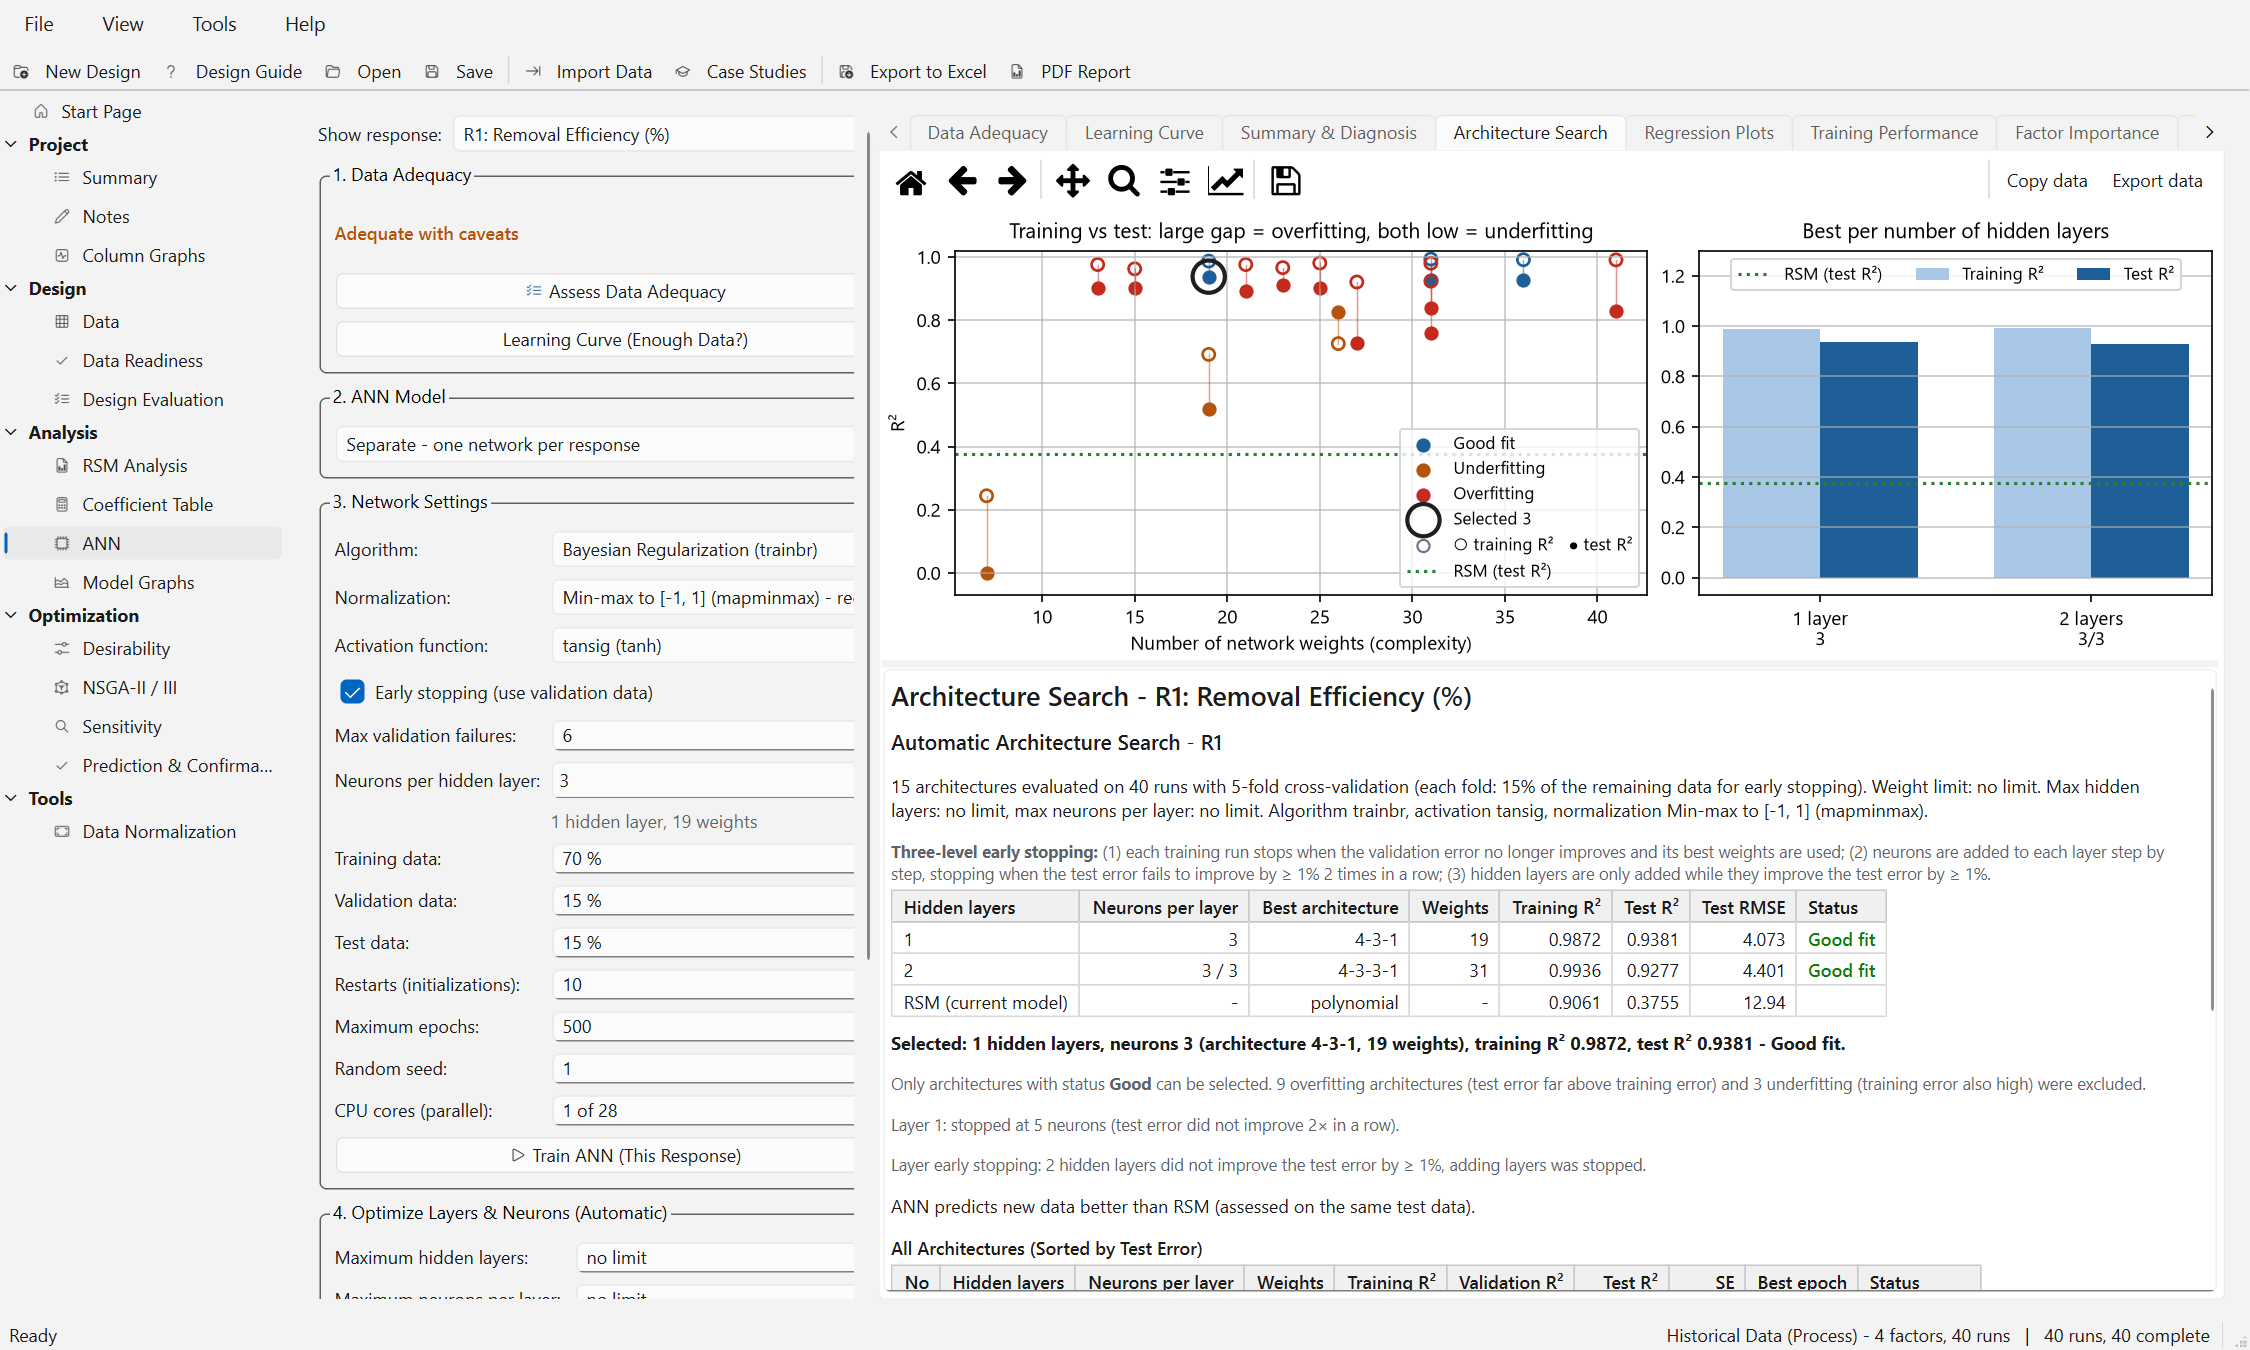
\includegraphics[width=\linewidth]{ann_search.png}
\caption{\ui{Architecture Search} tab for the dye adsorption case with the default settings: 15 candidate networks,
the selected 4-3-1 network (circled), the best network per depth and the RSM test $R^2$ of 0.3755 (dotted).}
\label{fig:ch07-search}
\end{figure}

\subsection{Example: dye adsorption}

With the default settings the search evaluates 15 architectures with 5-fold cross-validation in about 5~s on one
core. Table~\ref{tab:ch07-searchex} lists them in the order of evaluation.

\begin{table}[htbp]
\centering
\caption{All candidates of the architecture search for the dye case (5-fold cross-validation, NMSE averaged over the
folds). $^*$ = selected.}\label{tab:ch07-searchex}
\begin{tabular}{@{}lrrrrrrl@{}}
\toprule
Neurons & $W$ & $E_\text{tr}$ & $E_\text{te}$ & SE & Train $R^2$ & Test $R^2$ & Status \\
\midrule
1       &  7 & 0.7553 & 0.9990 & 0.2275 & 0.245 & 0.001 & Underfitting \\
2       & 13 & 0.0236 & 0.0974 & 0.0171 & 0.976 & 0.903 & Overfitting \\
3$^*$   & 19 & 0.0128 & 0.0619 & 0.0097 & 0.987 & 0.938 & Good fit \\
4       & 25 & 0.0187 & 0.0978 & 0.0263 & 0.981 & 0.902 & Overfitting \\
5       & 31 & 0.0194 & 0.1622 & 0.0652 & 0.981 & 0.838 & Overfitting \\
3/1     & 21 & 0.0237 & 0.1074 & 0.0473 & 0.976 & 0.893 & Overfitting \\
3/2     & 26 & 0.2738 & 0.1735 & 0.0587 & 0.726 & 0.827 & Underfitting \\
3/3     & 31 & 0.0064 & 0.0723 & 0.0158 & 0.994 & 0.928 & Good fit \\
3/4     & 36 & 0.0084 & 0.0726 & 0.0178 & 0.992 & 0.927 & Good fit \\
3/5     & 41 & 0.0089 & 0.1718 & 0.1276 & 0.991 & 0.828 & Overfitting \\
2/1     & 15 & 0.0372 & 0.0973 & 0.0178 & 0.963 & 0.903 & Overfitting \\
2/2     & 19 & 0.3080 & 0.4810 & 0.2682 & 0.692 & 0.519 & Underfitting \\
2/3     & 23 & 0.0335 & 0.0870 & 0.0114 & 0.967 & 0.913 & Overfitting \\
2/4     & 27 & 0.0789 & 0.2732 & 0.1003 & 0.921 & 0.727 & Overfitting \\
2/5     & 31 & 0.0762 & 0.2404 & 0.1518 & 0.924 & 0.760 & Overfitting \\
\bottomrule
\end{tabular}
\end{table}

The course of the search can be followed with the rules above:
\begin{itemize}
  \item Layer 1: 1, 2 and 3 neurons each improve the test error; 4 neurons (0.0978) and 5 neurons (0.1622) fail
    twice in a row, so growth stops at 5 neurons (``Layer 1: stopped at 5 neurons (test error did not improve 2×
    in a row).'').
  \item Layer 2 is grown on the two best one-layer networks, 3 and 2 neurons. The best two-layer network, 3/3,
    has $E_\text{te} = 0.0723$, which is not 1~\% below 0.0619, so no third layer is tried (``Layer early stopping:
    2 hidden layers did not improve the test error by $\ge$ 1\%, adding layers was stopped.'').
  \item With $E^* = 0.0619$, the network with 2 neurons is classified as overfitting: its test error 0.0974 is
    more than twice its training error 0.0236 and more than $1.2E^* = 0.0743$. One neuron is underfitting
    ($E_\text{tr} = 0.755$). Nine candidates are overfitting, three underfitting and three good.
  \item 1-SE rule: $\tau = 0.0619 + \max(0.0097, 0.002) = 0.0716$. The good networks 3/3 (0.0723) and 3/4 (0.0726)
    are just above $\tau$, so the selected network is the best raw one, 4-3-1 with 19 weights (training $R^2$
    0.9872, test $R^2$ 0.9381).
  \item RSM on the same folds: training $R^2$ 0.9061, test $R^2$ 0.3755 (test RMSE 12.94 against 4.073 for the
    ANN), so ``ANN predicts new data better than RSM''. The four-factor quadratic model cannot follow the pH
    optimum and the saturation of this response.
\end{itemize}

\section{Fit diagnosis after a search}\label{sec:ch07-diagnosis}

The \ui{Summary \& Diagnosis} tab (Figure~\ref{fig:ch07-summary}) starts with the architecture, the algorithm, the
number of weights, the normalization, the data split, the number of epochs with the stop reason, the effective
parameters $\gamma$ (trainbr) and the number of restarts. The \ui{Fit Diagnosis} follows.
\begin{itemize}
  \item \emph{After an architecture search}, the headline is the cross-validated status of the selected
    candidate, for example ``Good fit (result of 5-fold cross-validation during architecture search)'', with the
    training, validation and test $R^2$ averaged over the folds. The section \ui{Single Train/Test Split (Final
    Model)} then gives the status of the final network on its one random split as secondary information, with the
    reason (``Single split: \dots''). The suggestions (reduce or add neurons, run the search) follow the
    cross-validated status.
  \item \emph{After training by hand}, the only status is that of the single split, marked ``(single train/test
    split)''.
  \item If the validation and test sets together have fewer than 10 runs, a note warns that the single-split
    diagnosis is uncertain.
  \item A table gives $R^2$ and NMSE of the single split for training, validation and test data (and the
    measurement noise limit $1-\nu$ when replicates exist), followed by the epoch whose weights were used, the
    stop reason and the criteria of both diagnoses.
\end{itemize}
Further down are the run numbers of each set (\ui{Data Split (Random, Automatic)}), the \ui{Performance} table
(Eq.~\eqref{eq:ch07-metrics}), an \ui{RSM vs ANN Comparison} on all data and on the ANN test runs, the relative
factor importance, and a red warning if the network has more weights than training targets.

Note that in the \ui{RSM vs ANN Comparison} on this tab, RSM was fitted on all runs, including the ANN test runs,
which favors RSM. The fair comparison is the one on the \ui{Architecture Search} tab or the RSM Predicted $R^2$,
as the note under the table says.

\paragraph{Example.} For the final 4-3-1 network of the dye case (Figure~\ref{fig:ch07-summary}), the split is 28
training, 6 validation and 6 test runs. Training stopped at epoch 20 by early stopping; the weights of epoch 7
were used. The headline is ``Good fit'' from 5-fold cross-validation (training $R^2$ 0.9872, validation 0.9313,
test 0.9381). On the single split the status is ``Overfitting'': training NMSE 0.0215, validation 0.0105, test
0.1466, and $(0.0105+0.1466)/2 = 0.079$ is 3.6 times the training error. Six test runs are too few to decide this:
one or two poorly predicted runs triple the test error. The cross-validated result, which uses every run once as a
test run, is the reliable one. Because epoch 7 lies inside the warm-up of 15 epochs, the first line reads
``effective parameters $\gamma$ not estimated yet (best epoch 7 lies within the warm-up; $\gamma$ is first
estimated after epoch 15)''.

\begin{figure}[htbp]
\centering
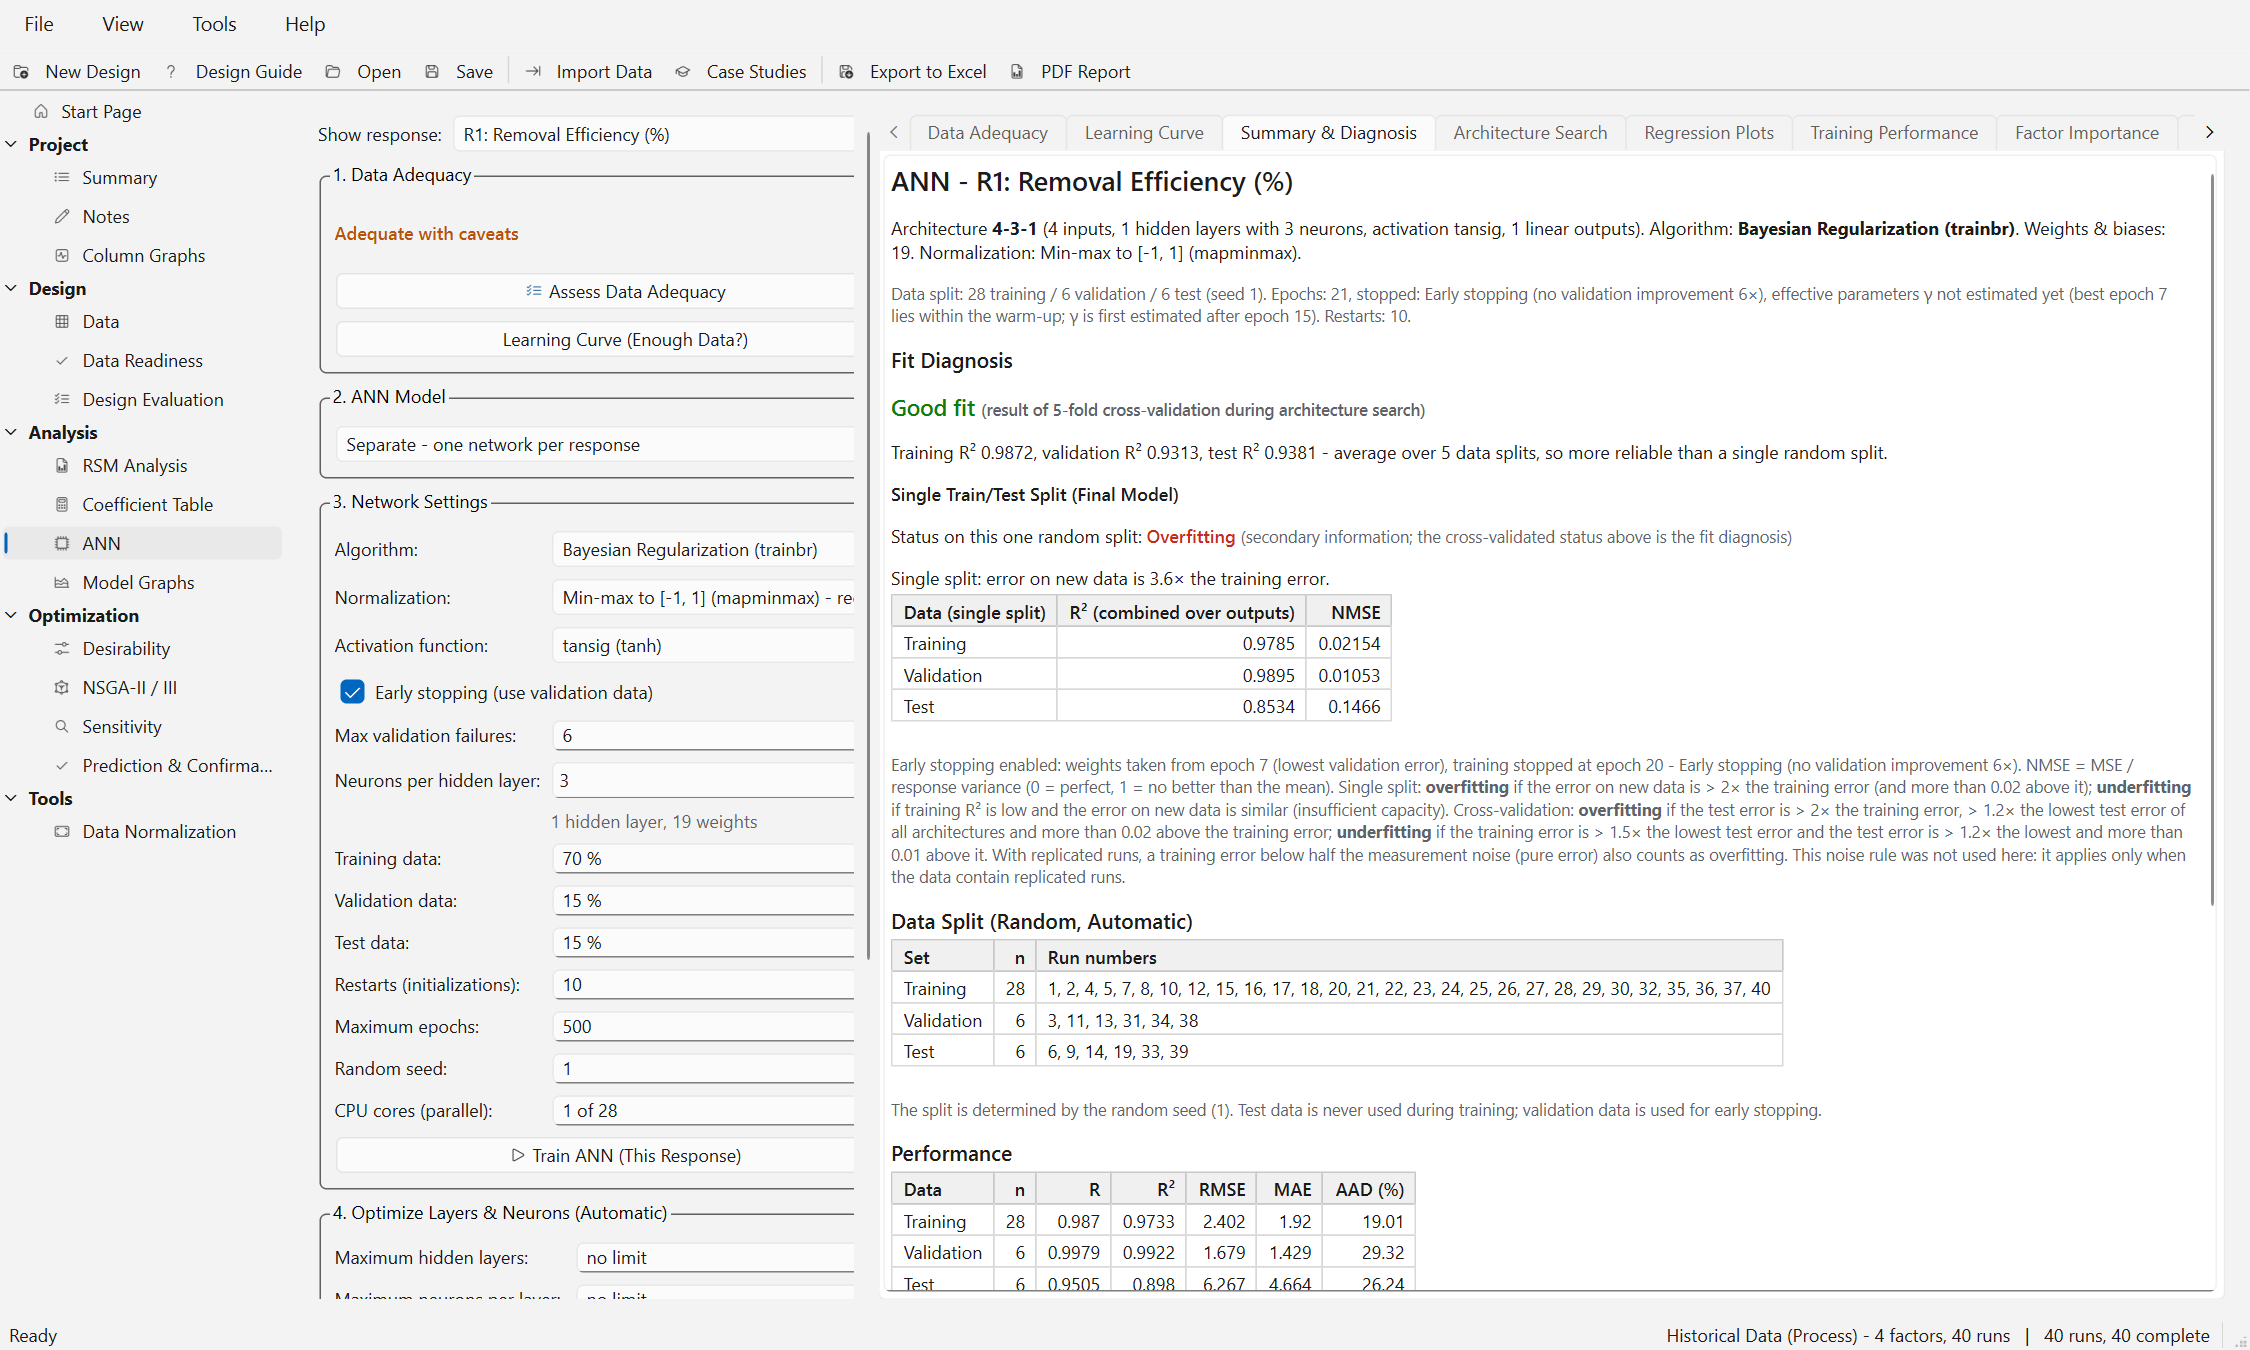
\includegraphics[width=\linewidth]{ann_summary.png}
\caption{\ui{Summary \& Diagnosis} tab of the selected 4-3-1 network: cross-validated ``Good fit'' as the headline,
the single split shown separately as ``Overfitting'', and the data split and performance tables.}
\label{fig:ch07-summary}
\end{figure}

\paragraph{When the diagnosis is poor.} \emph{Underfitting} (both errors high): allow more neurons or layers
(remove limits), increase \ui{Maximum epochs:} or \ui{Restarts (initializations):}, or check that the response is
not dominated by noise. \emph{Overfitting} (cross-validated): use trainbr with early stopping, set a weight limit,
or add runs; if every network overfits, the data are too few for an ANN and RSM is the better choice.
\emph{Cross-validated good fit but single split overfitting}: accept the cross-validated result, but expect
predictions with an error near the test RMSE of the search (4.07 in the example), not the training RMSE.

\section{Check B: learning curve}\label{sec:ch07-learning}

\paragraph{Purpose.} The learning curve answers ``Would more runs still improve the network, and roughly how
many?''. The network is trained on growing subsets of the data and tested on runs that are never used for
training. If the test $R^2$ still rises at the full data size, more runs would help; if it has flattened, the
remaining error comes from noise or from the model, not from the amount of data.

\subsection{How to use}

\begin{enumerate}
  \item Select the response and click \ui{Learning Curve (Enough Data?)}. The response must be continuous and have
    at least 12 complete runs.
  \item The network size is that of the response's trained network (its layers, activation, algorithm and
    normalization); without one, the entry \ui{Neurons per hidden layer:} and the current settings are used. A
    network that was switched to Adam automatically is trained with trainbr. The seed is \ui{Random seed:}.
  \item The \ui{Learning Curve} tab opens and the status line reads, for example, ``Learning curve finished: more
    data would still help (run estimate unreliable)''.
\end{enumerate}
Every point of the curve uses fixed settings that do not depend on \ui{Network Settings}: 2 restarts, at most 300
epochs, early stopping after 6 validation failures, and the trainbr convergence test.

\subsection{Procedure as implemented}

\begin{enumerate}
  \item The number of repeats is $R = 10$ for $N < 60$, 6 for $N < 400$ and 4 otherwise.
  \item In each repeat, $n_\text{te} = \max(3, \operatorname{round}(0.2N))$ runs are drawn as a fixed test set; the
    other runs form the pool.
  \item For the fractions $f = 0.3, 0.4, \dots, 1.0$ of the pool, the first $n = \max(5, \operatorname{round}(f\,
    n_\text{pool}))$ runs of the shuffled pool are used for fitting (nested subsets). Of these, $\max(1,
    \operatorname{round}(0.15\,n))$ are validation runs when $n \ge 10$. The network is trained on the subset and
    its NMSE on the fixed test set is recorded (with the variance of all runs in the denominator).
  \item The current RSM model is fitted on the same subsets and tested on the same runs; subsets too small for its
    terms give no value.
  \item For each size the median and the quartiles over the repeats are shown.
\end{enumerate}

\subsection{Power-law fit and runs needed}

The median test NMSE is fitted with the power law
\begin{equation}
  e(n) = a + b\,n^{-c}, \qquad a, b \ge 0, \label{eq:ch07-powerlaw}
\end{equation}
which is a common model of learning curves \citep{figueroa2012}. Here $a$ is the error that would remain with
unlimited data, so $R^2_\infty = 1 - a$ is the upper limit of the test $R^2$. The exponent is searched on the grid
$c = 0.20, 0.25, \dots, 2.50$ (47 values); for each $c$, $a$ and $b$ are found by least squares (with $a = 0$ and
$b$ refitted if $a$ would be negative), and the $c$ with the smallest residual sum of squares is kept. When there
are at least six sizes, the two smallest are left out of the fit because they are too noisy.

The number of fitting runs at which the test $R^2$ comes within $0.01$ of its limit is
\begin{equation}
  b\,n^{*\,-c} = 0.01 \quad\Longrightarrow\quad n^* = \left\lceil \left(\frac{b}{0.01}\right)^{1/c}\right\rceil.
  \label{eq:ch07-nstar}
\end{equation}
To express its uncertainty, the repeats are resampled 200 times (bootstrap), the median curve is refitted and
$n^*$ recomputed each time. The reported value $n^*_\text{med}$ is the median of the bootstrap values, with their
quartiles as the range. Since $n^*$ counts runs used for fitting, the total number of runs including the test
share is
\begin{equation}
  N_\text{total} = \left\lceil \frac{n^*_\text{med}}{1 - n_\text{te}/N} \right\rceil. \label{eq:ch07-ntotal}
\end{equation}

\subsection{Statuses and messages}

With $n_\text{full}$ the largest subset of the curve:
\begin{itemize}
  \item $n^*_\text{med} \le n_\text{full}$: ``\textbf{The data is sufficient.} The curve has flattened \dots''.
  \item $n_\text{full} < n^*_\text{med} \le 5\,n_\text{full}$: ``\textbf{More data would still help.} \dots{}
    Estimate: about $N_\text{total}$ runs in total (range \dots; add about \dots{} runs) \dots''. This is an
    extrapolation: add runs in stages (for example half first) and repeat the learning curve.
  \item $n^*_\text{med} > 5\,n_\text{full}$: ``\textbf{The data is still far from sufficient.}'' The message states
    the test used (more than 5 times the largest training set, that is more than $5N$ runs in total) and suggests
    RSM, fewer factors or narrower ranges.
  \item $N < 25$ overrides the status: ``\textbf{Too little data (\dots{} runs) for a reliable learning curve.}''
    The subsets are then too small to show a trend.
\end{itemize}
A reliability warning is added (``The run estimate is unreliable: \dots'') when the fitted exponent lies at the
edge of the grid ($c = 0.2$ or $2.5$), when the fitted error limit is $a = 0$ (the curve predicts a perfect fit with
unlimited data), or when the interquartile range of the bootstrap estimate is very wide (upper/lower quartile $>
3$). The estimate is not changed; it should then be read only as an indication of \emph{whether} more runs help,
not \emph{how many}.

The report ends with the ANN and RSM test $R^2$ at the full size (``RSM usually wins with little data; ANN needs
more data to catch up'' when RSM is better) and a table per size: training data, ANN test $R^2$ (median and
quartiles), ANN training $R^2$ and RSM test $R^2$. The plot shows the median test $R^2$ with an interquartile band,
the training $R^2$ (dashed), the RSM test $R^2$ (squares), and, for the statuses ``more'' and ``enough'', the
fitted curve and the estimated upper limit; for ``more'' a vertical line marks $n^*$.

\subsection{Example: dye adsorption}

Figure~\ref{fig:ch07-learning} shows the learning curve computed with the default entry of 5 neurons (before the
search). With $N = 40$ there are 10 repeats, 8 fixed test runs and fitting subsets of 10, 13, 16, 19, 22, 26, 29
and 32 runs. The median test $R^2$ rises from $-0.014$ at 10 runs to 0.898 at 26 runs and 0.876 at 32 runs; RSM
reaches only 0.429 at 32 runs and is strongly negative below 19 runs, where the 15 coefficients of the four-factor
quadratic model are barely or not estimable. The power-law fit (on the six largest sizes) gives $a = 0$, $b =
509.3$ and $c = 2.5$, so $R^2_\infty = 1.000$ and, from Eq.~\eqref{eq:ch07-nstar}, $(509.3/0.01)^{1/2.5} = 76.3$,
that is 77 runs; the bootstrap median is $n^*_\text{med} = 80$ (quartiles 76 and 88). With $n_\text{te}/N = 0.2$,
$N_\text{total} = 80/0.8 = 100$ runs (range 95 to 111), so about 60 runs should be added. Because $c$ lies at the
upper edge of the grid and $a = 0$, the report flags the estimate as unreliable. The sound conclusion is
qualitative: the ANN is still improving at 40 runs and more runs would help, but the number 100 should not be
taken literally. The plateau between 26 and 32 runs shows how noisy the curve is at this size.

\begin{figure}[htbp]
\centering
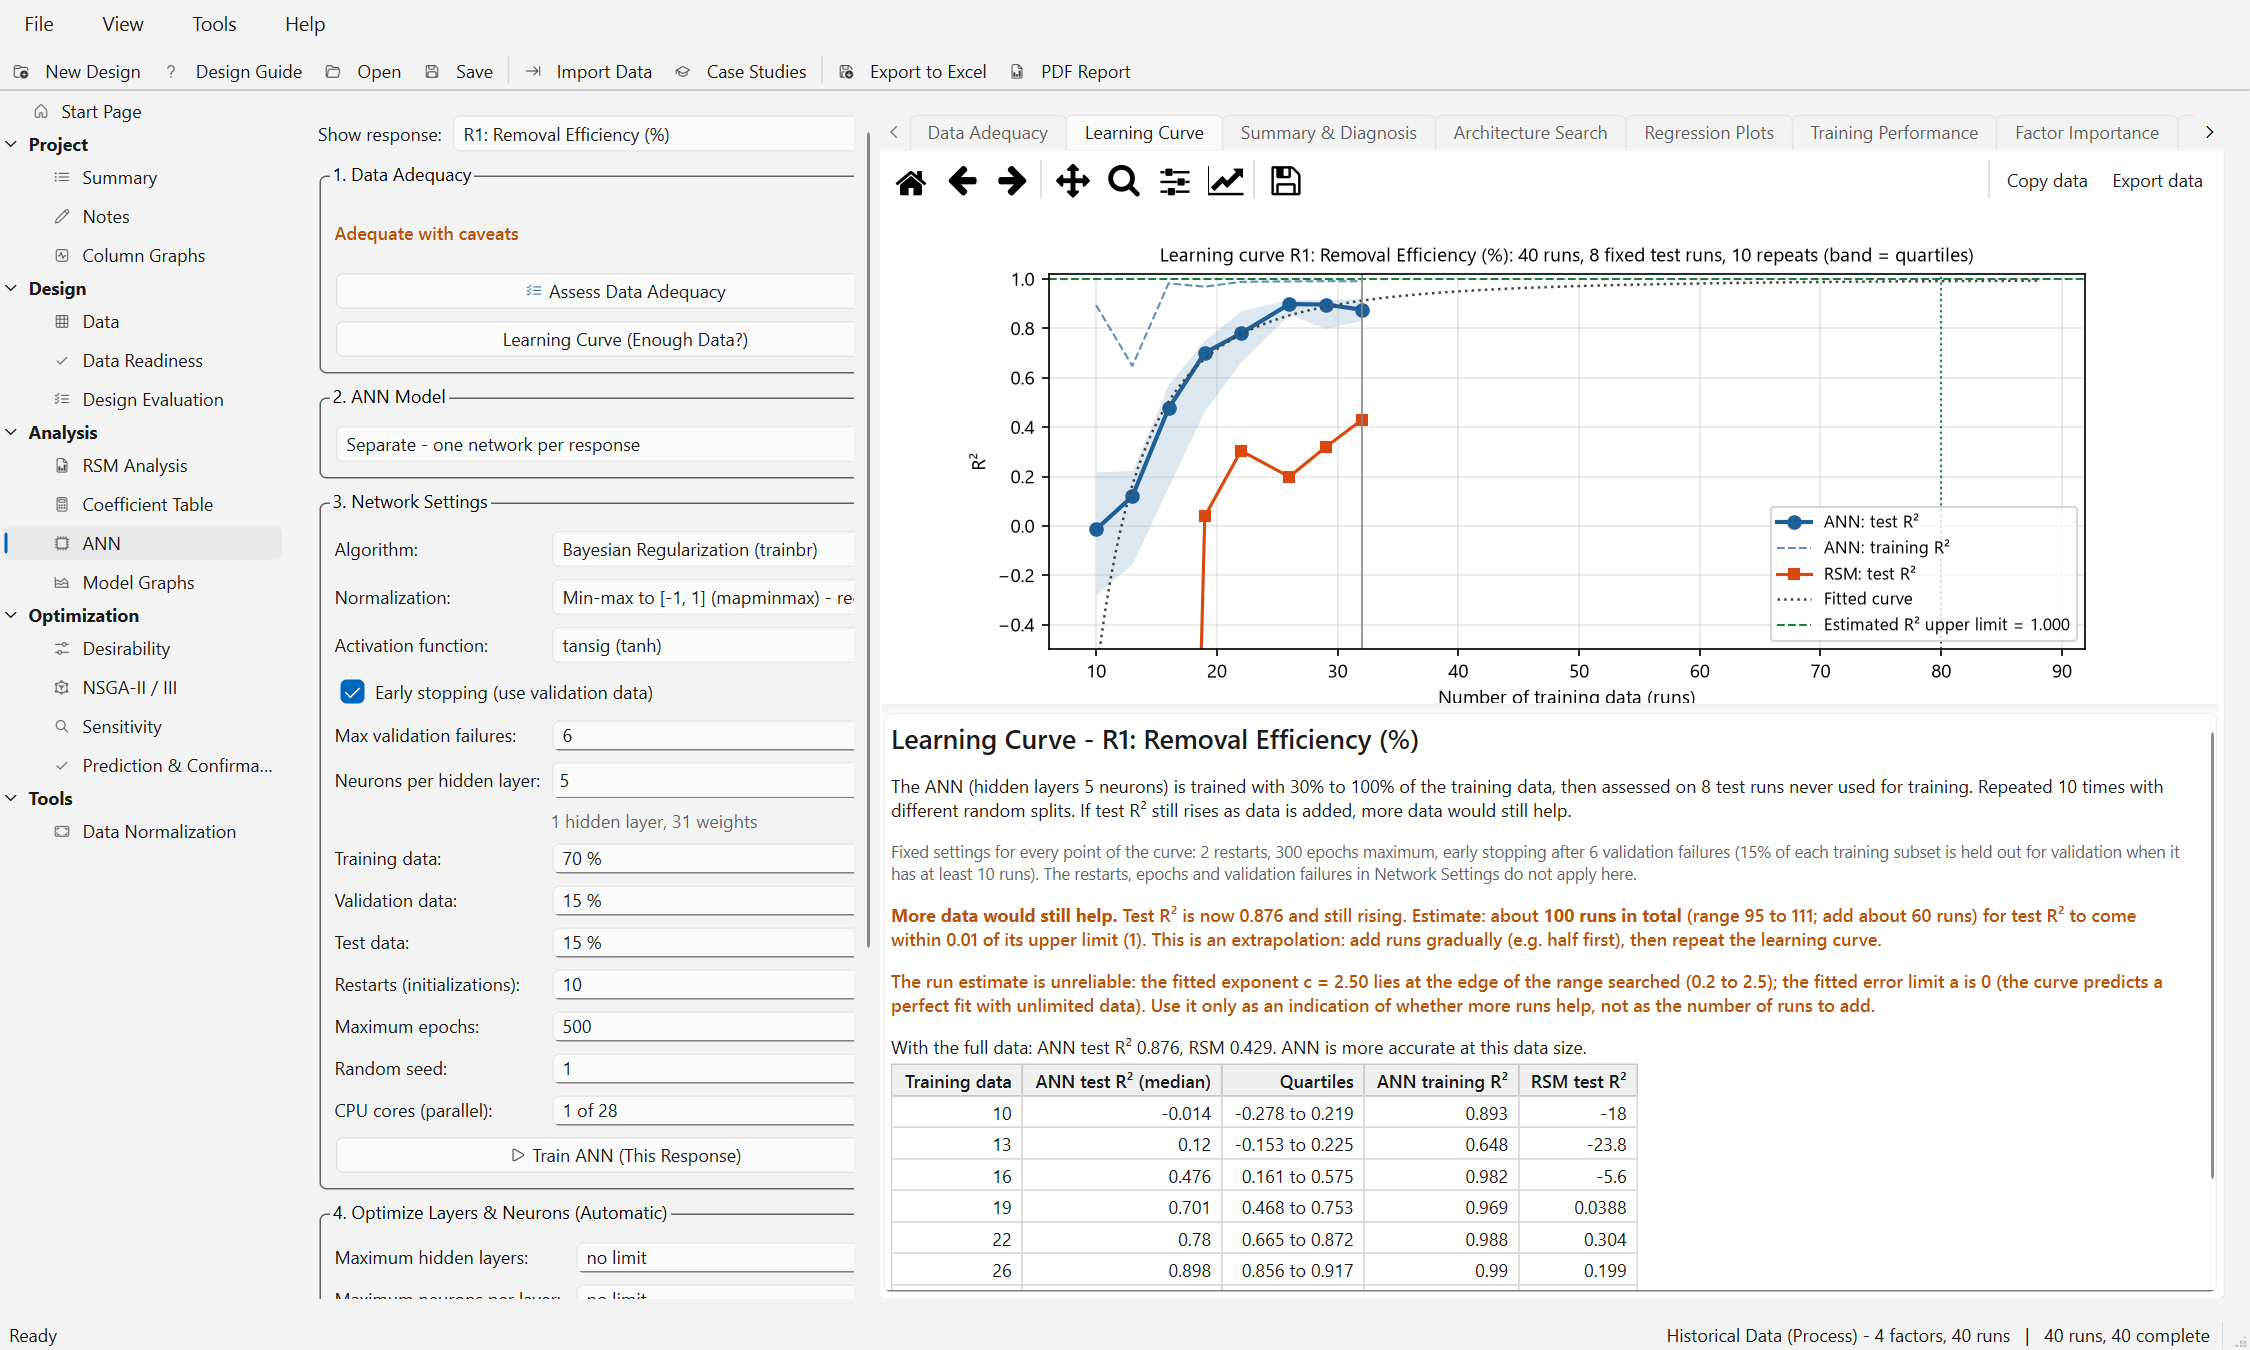
\includegraphics[width=\linewidth]{ann_learning_curve.png}
\caption{\ui{Learning Curve} tab for the dye case (1 hidden layer of 5 neurons): ANN test $R^2$ with interquartile
band, training $R^2$, RSM test $R^2$, fitted power law with the estimated upper limit and the line at $n^* = 80$
training runs; below, the message ``More data would still help'' with the reliability warning.}
\label{fig:ch07-learning}
\end{figure}

\paragraph{Limitations.} The curve depends on the network size used; run it with the network selected by the
search when available. Extrapolating a power law fitted on a handful of noisy points is uncertain, which is why the
bootstrap range and the warnings are shown. New runs should cover the factor space (the \ui{Data Readiness} page
suggests space-filling runs); runs repeated at existing points add little information for an ANN.

\section{Other result tabs}\label{sec:ch07-tabs}

\paragraph{Regression Plots.} Four panels (Training, Validation, Test, All) plot the network output against the
target with the 1:1 line (dotted) and a least-squares line; the title of each panel gives the correlation $R$
(Figure~\ref{fig:ch07-regression}). Points of the test panel far from the line are the runs the network predicts
poorly. For the dye network $R$ is 0.9870 (training), 0.9979 (validation), 0.9505 (test) and 0.9809 (all data).

\begin{figure}[htbp]
\centering
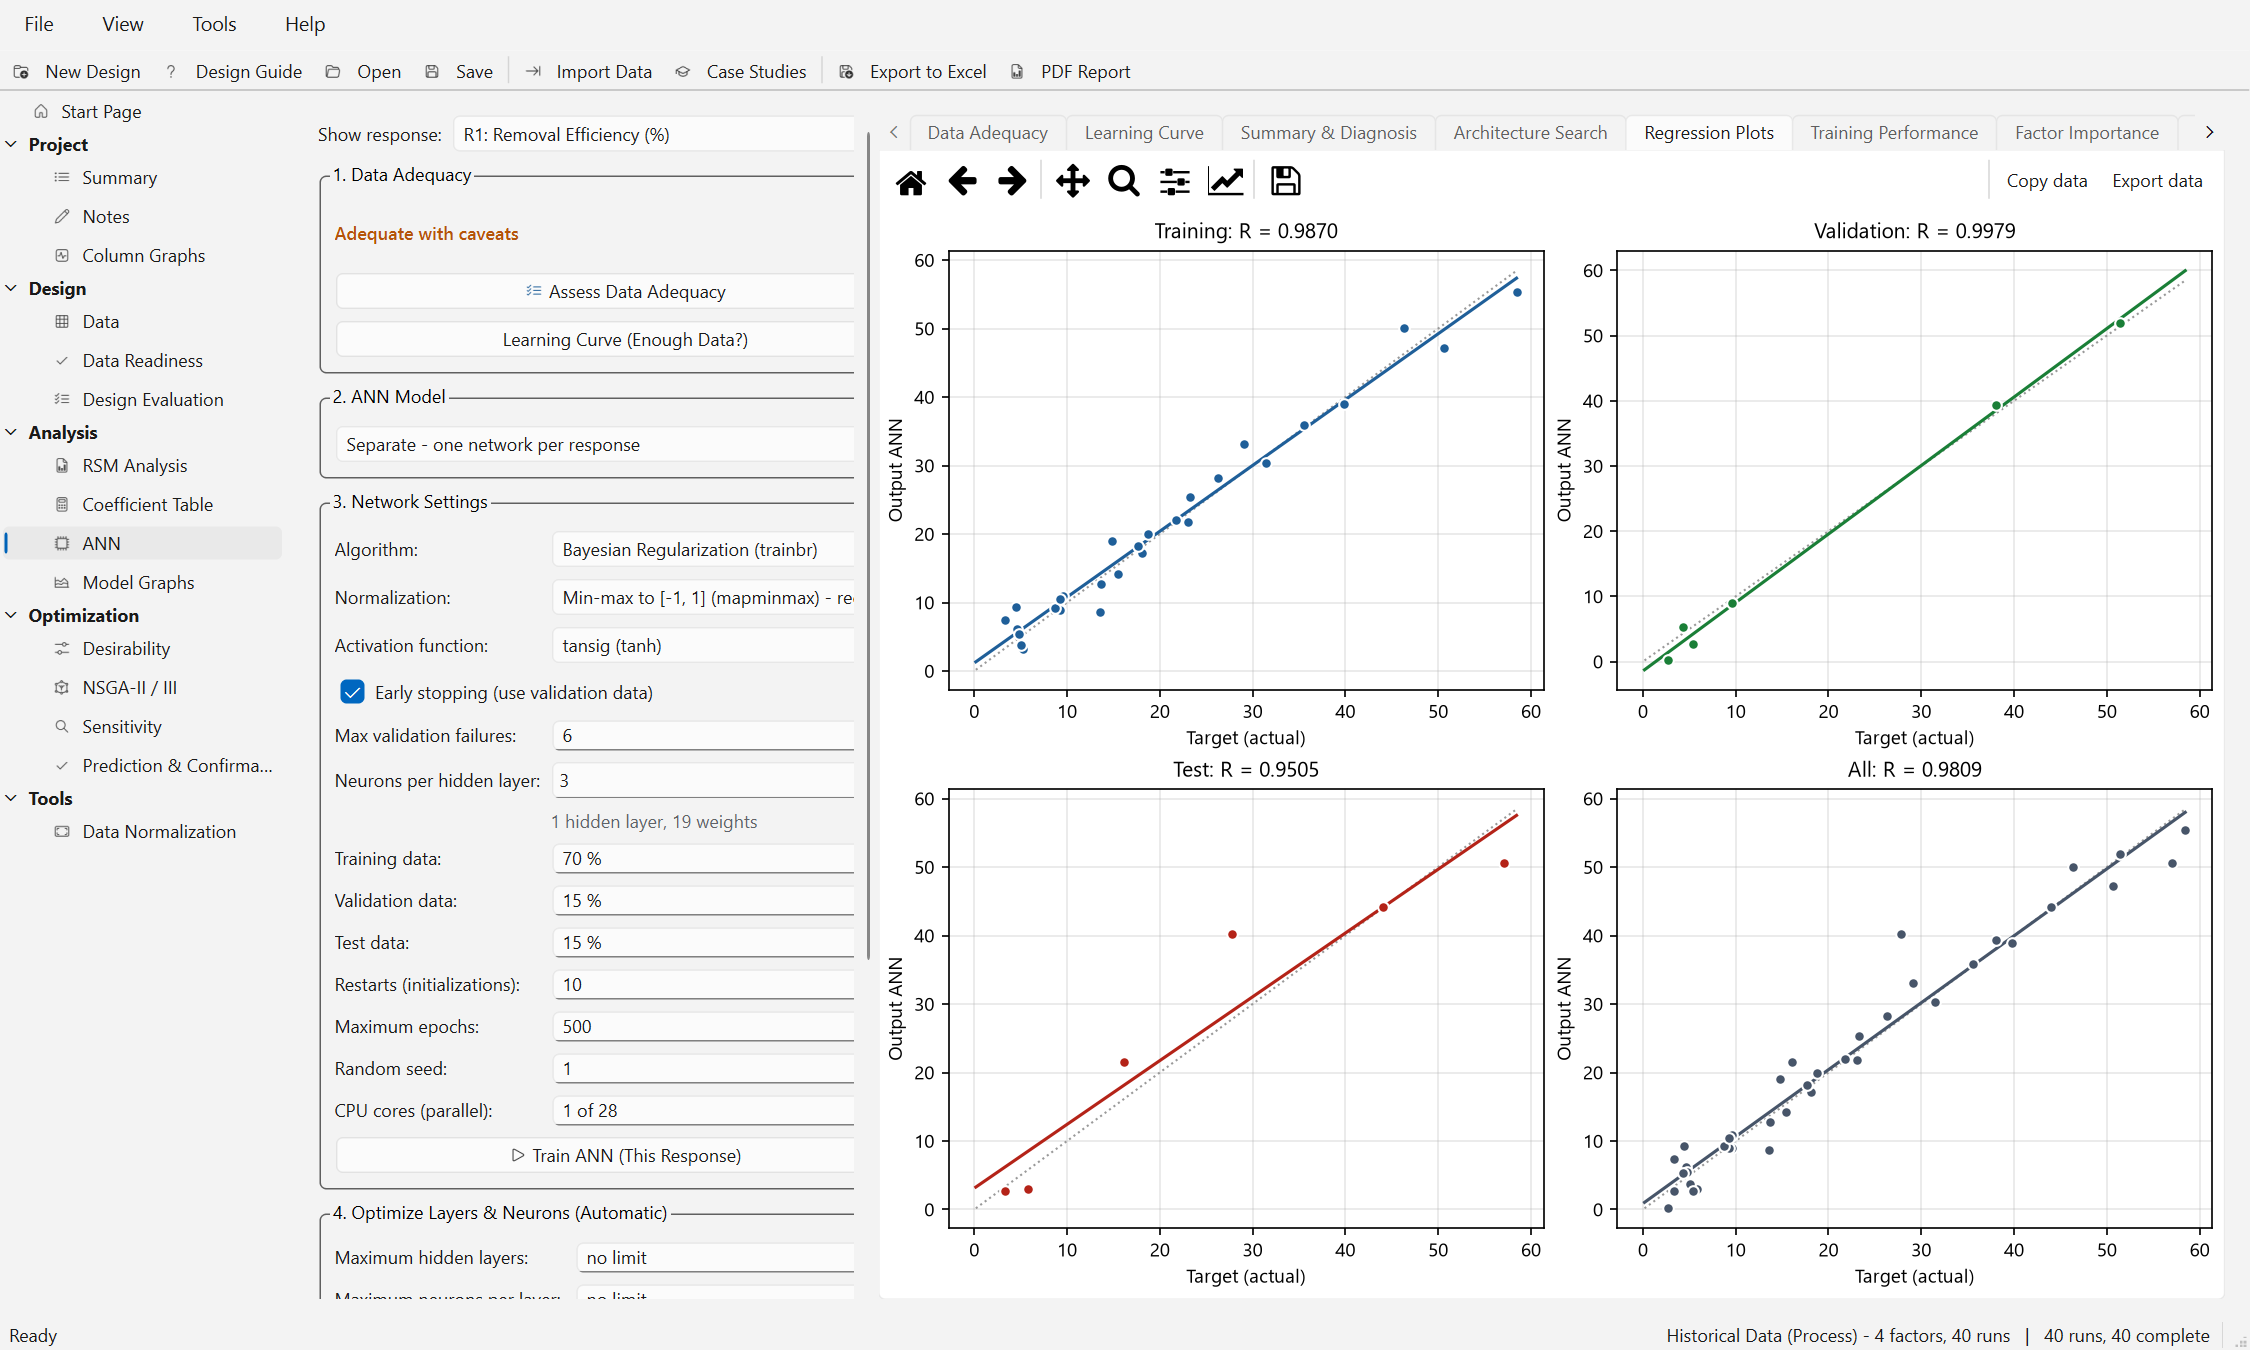
\includegraphics[width=\linewidth]{ann_regression.png}
\caption{\ui{Regression Plots} of the 4-3-1 network for training, validation, test and all data.}
\label{fig:ch07-regression}
\end{figure}

\paragraph{Training Performance.} The mean squared error on the normalized scale per epoch for training,
validation and test data, on a logarithmic axis (Figure~\ref{fig:ch07-performance}). A dotted vertical line marks
the epoch whose weights are used (``Weights used (epoch 7) - early stopping'') and a shaded band marks the epochs in
which the validation error did not improve. In the dye example the validation error reaches its minimum at epoch
7; with trainbr, failures are counted only from epoch 15, so training stops at epoch 20. A test curve that keeps
rising after the marked epoch is the typical picture that early stopping prevents.

\begin{figure}[htbp]
\centering
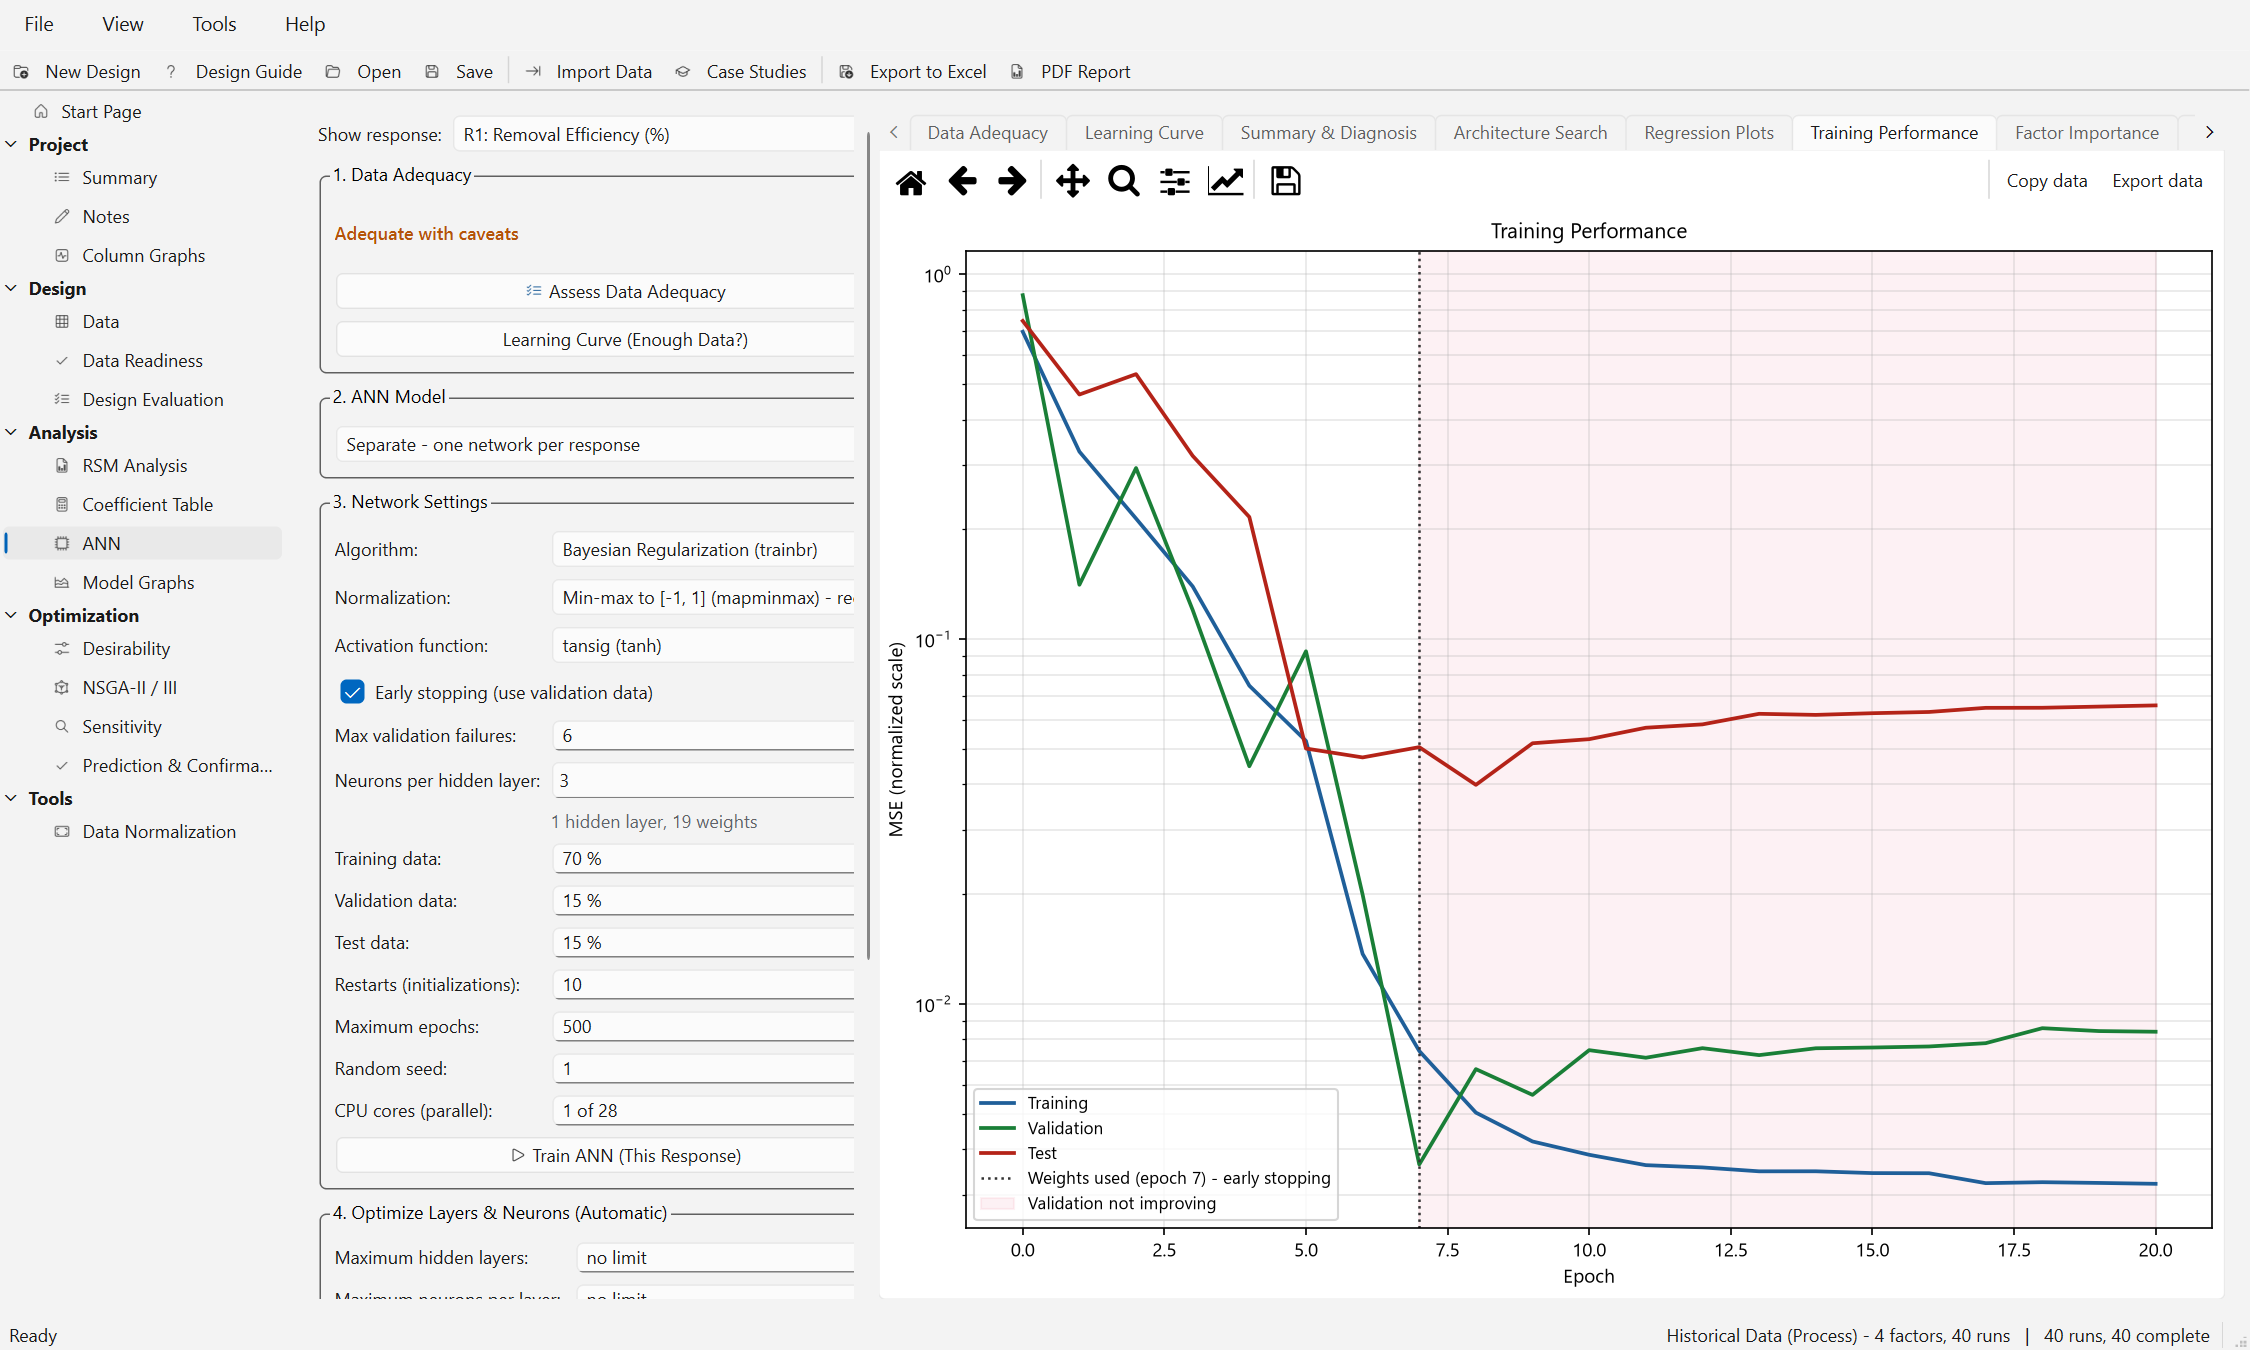
\includegraphics[width=\linewidth]{ann_performance.png}
\caption{\ui{Training Performance} of the 4-3-1 network: the weights of epoch 7 (lowest validation error) are used;
the shaded band shows the epochs without validation improvement.}
\label{fig:ch07-performance}
\end{figure}

\paragraph{Factor Importance.} The relative importance of each factor follows Garson's method as described by
\citet{goh1995}, extended to several hidden layers. With the absolute input weights of each first-layer neuron
normalized to shares,
\begin{equation}
  S^{(1)}_{hi} = \frac{|W^{(1)}_{hi}|}{\sum_{i'} |W^{(1)}_{hi'}|}, \qquad
  S^{(l)} = \bar{A}^{(l)} S^{(l-1)}, \quad \bar{A}^{(l)}_{hg} = \frac{|W^{(l)}_{hg}|}{\sum_{g'}|W^{(l)}_{hg'}|},
  \label{eq:ch07-garson1}
\end{equation}
and $v_h$ the weights from the last hidden layer to the output shown, the importance of input $i$ is
\begin{equation}
  I_i = \sum_{h} \frac{|v_h|}{\sum_{h'}|v_{h'}|}\, S^{(L)}_{hi}. \label{eq:ch07-garson2}
\end{equation}
For one hidden layer this is the classic Garson formula; for more layers (``Garson extended to multiple hidden
layers'') each input's share is passed through every layer in proportion to the absolute weights. The values of
the one-hot columns of a categorical factor are added, and the result is scaled to 100~\%. For the dye network the
order is pH 68.2~\%, Initial Concentration 13.3~\%, Contact Time 11.1~\% and Adsorbent Dose 7.4~\%
(Figure~\ref{fig:ch07-importance}), consistent with the strong pH optimum of this system. Garson's method uses only
weight magnitudes: it shows neither the direction of an effect nor whether it is linear, and it becomes
unreliable when factors are correlated. Use the model graphs or the sensitivity study for the shape of the
effects.

\begin{figure}[htbp]
\centering
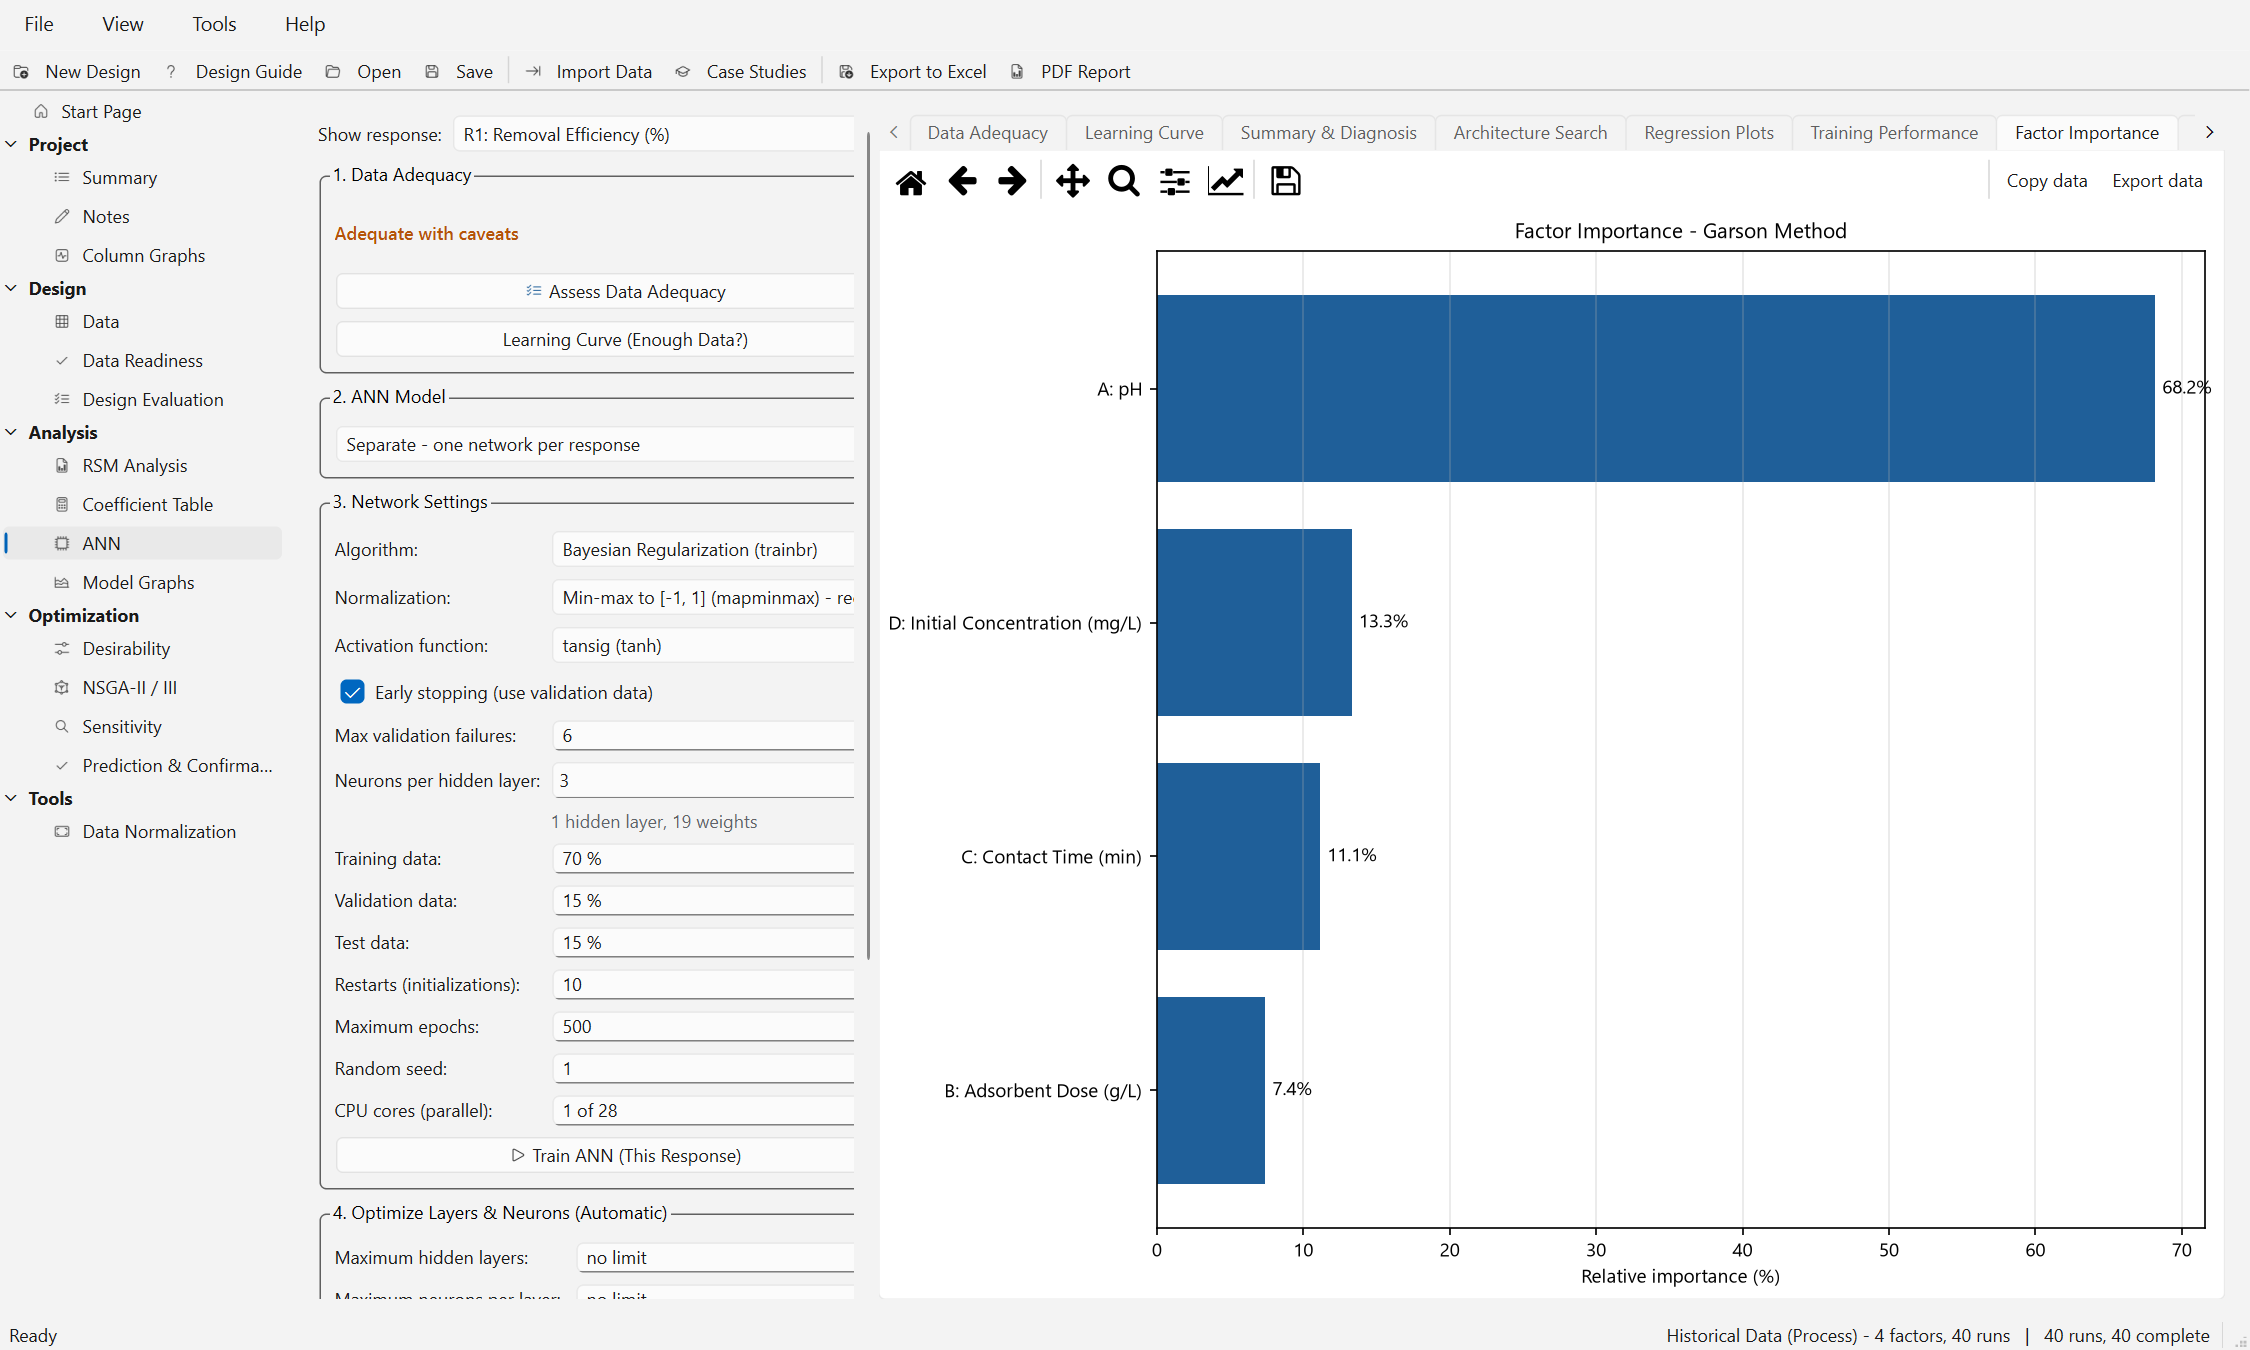
\includegraphics[width=\linewidth]{ann_importance.png}
\caption{\ui{Factor Importance} (Garson method) of the 4-3-1 network.}
\label{fig:ch07-importance}
\end{figure}

\paragraph{RSM vs ANN.} The left panel plots predicted against actual values for both models on all runs (RSM as
squares, ANN as dots, each with its $R^2$); the right panel shows the residual (actual $-$ predicted) per run in
standard order. In the dye case (Figure~\ref{fig:ch07-rsmann}) RSM reaches $R^2$ 0.8769 with residuals up to about
$+16$ and even a negative prediction, while the ANN reaches 0.9614 and stays within about $\pm 6$ except for one
run. Both values are on the data used for fitting (the RSM on all runs); judge predictive accuracy by the
cross-validated values of the search.

\begin{figure}[htbp]
\centering
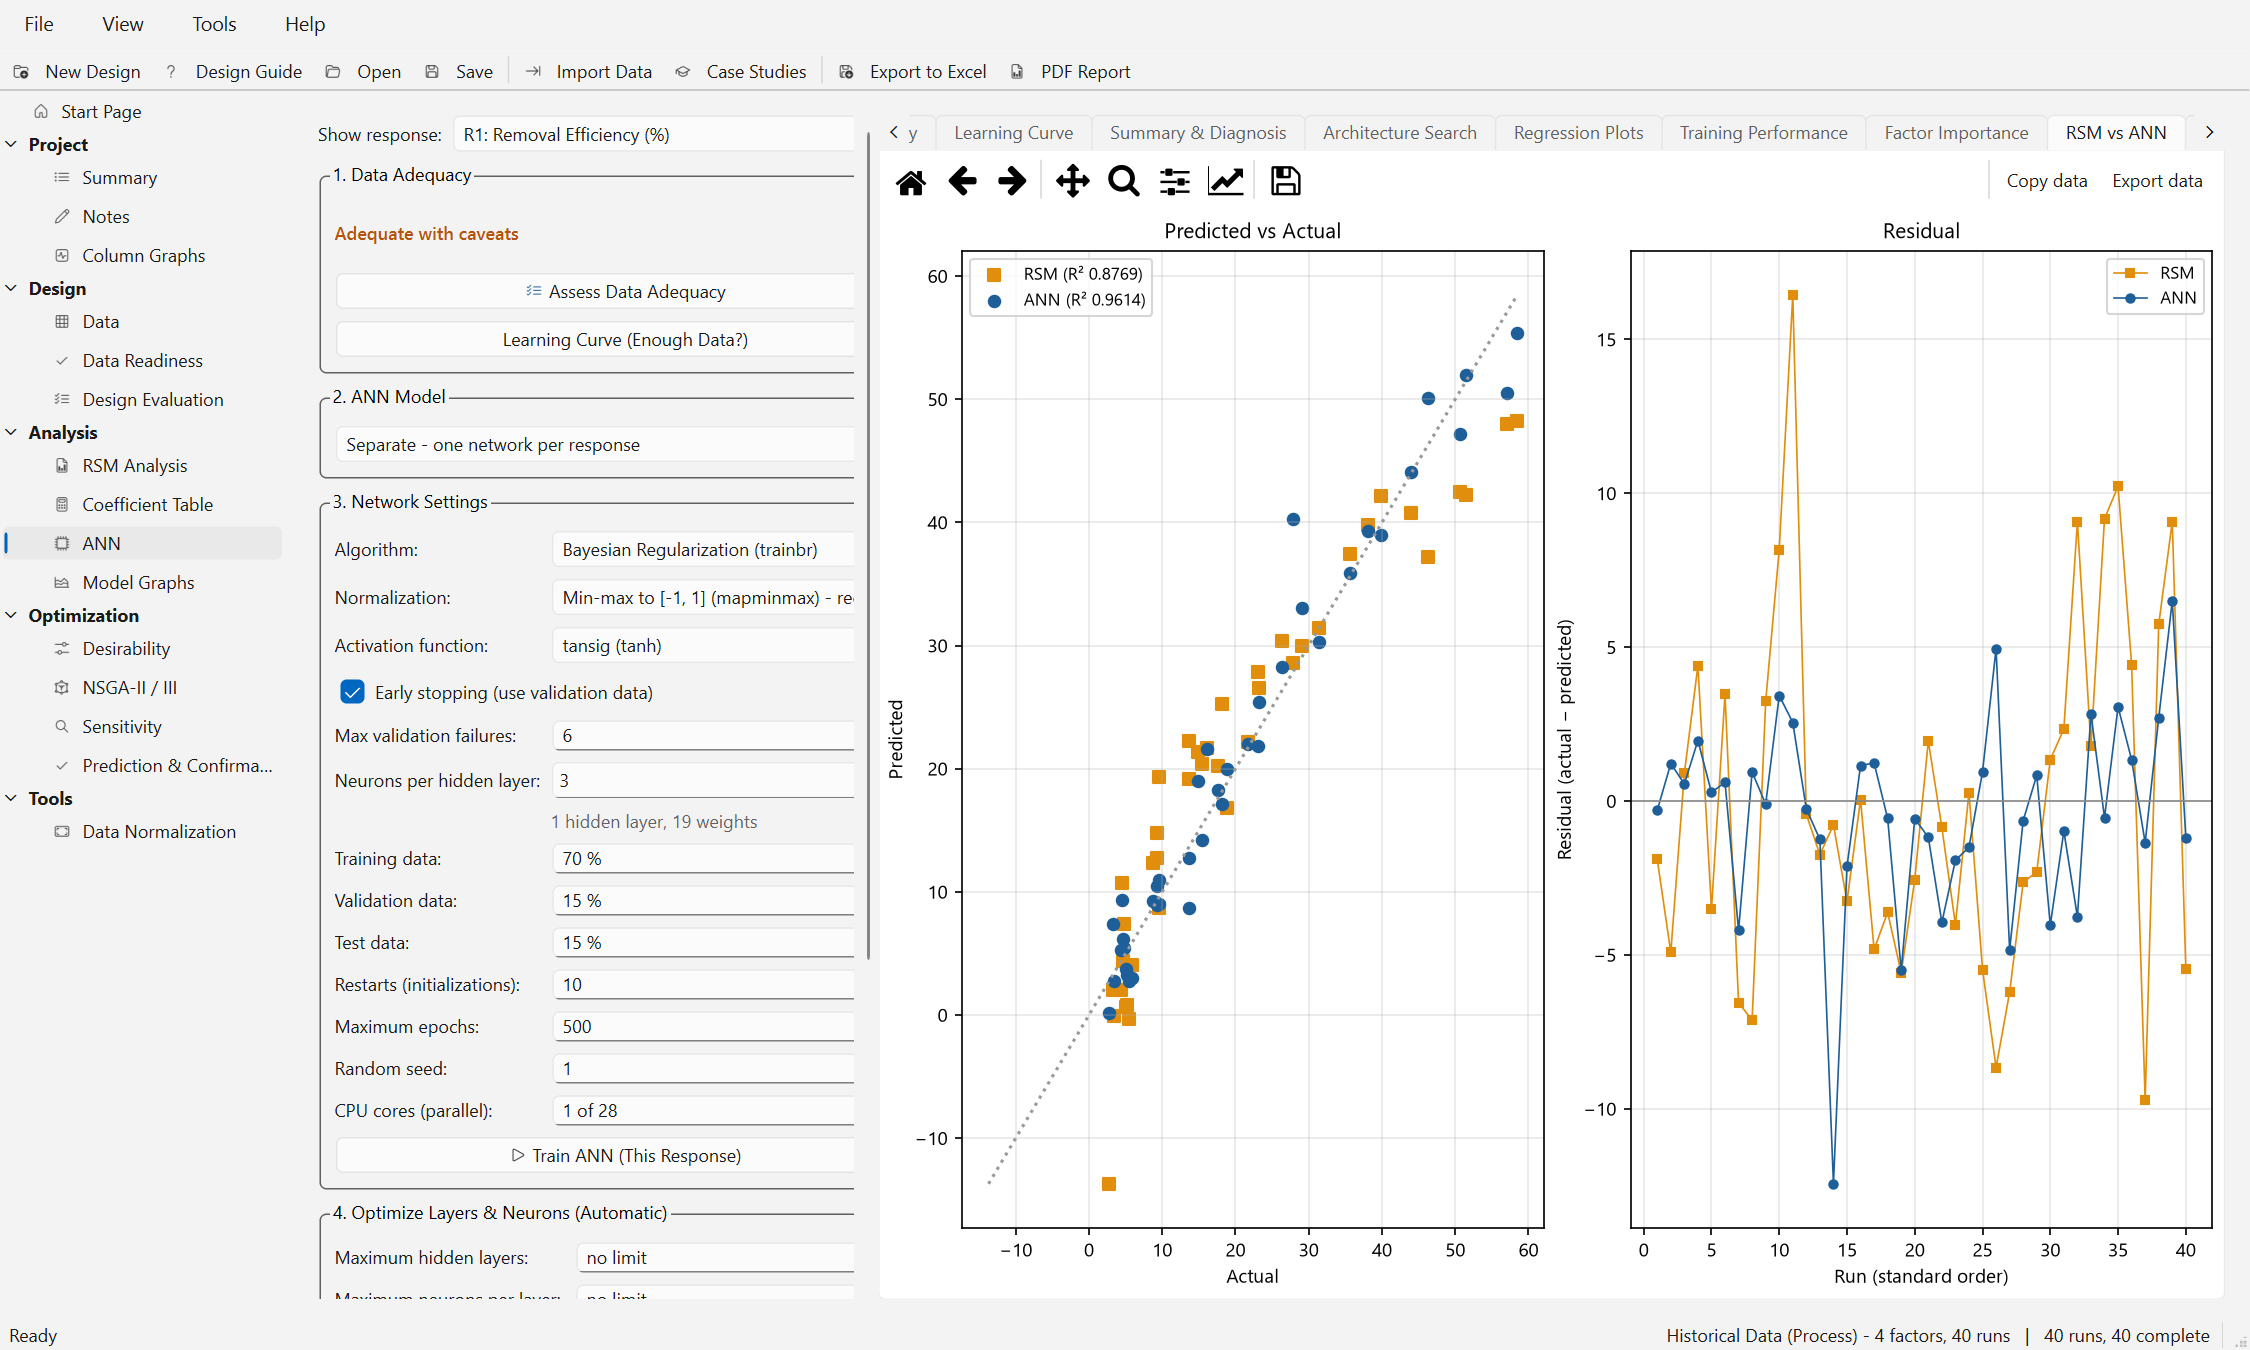
\includegraphics[width=\linewidth]{ann_rsm_vs_ann.png}
\caption{\ui{RSM vs ANN} tab for the dye case: predicted against actual values and residuals per run.}
\label{fig:ch07-rsmann}
\end{figure}

\paragraph{Network Diagram.} Inputs on the left, one column per hidden layer (``Hidden $i$ ($n$ neurons, tansig)''),
linear outputs on the right (Figure~\ref{fig:ch07-diagram}). Blue lines are positive weights, red lines negative;
thickness and opacity grow with $|w|$. In a combined network the output shown is highlighted.

\begin{figure}[htbp]
\centering
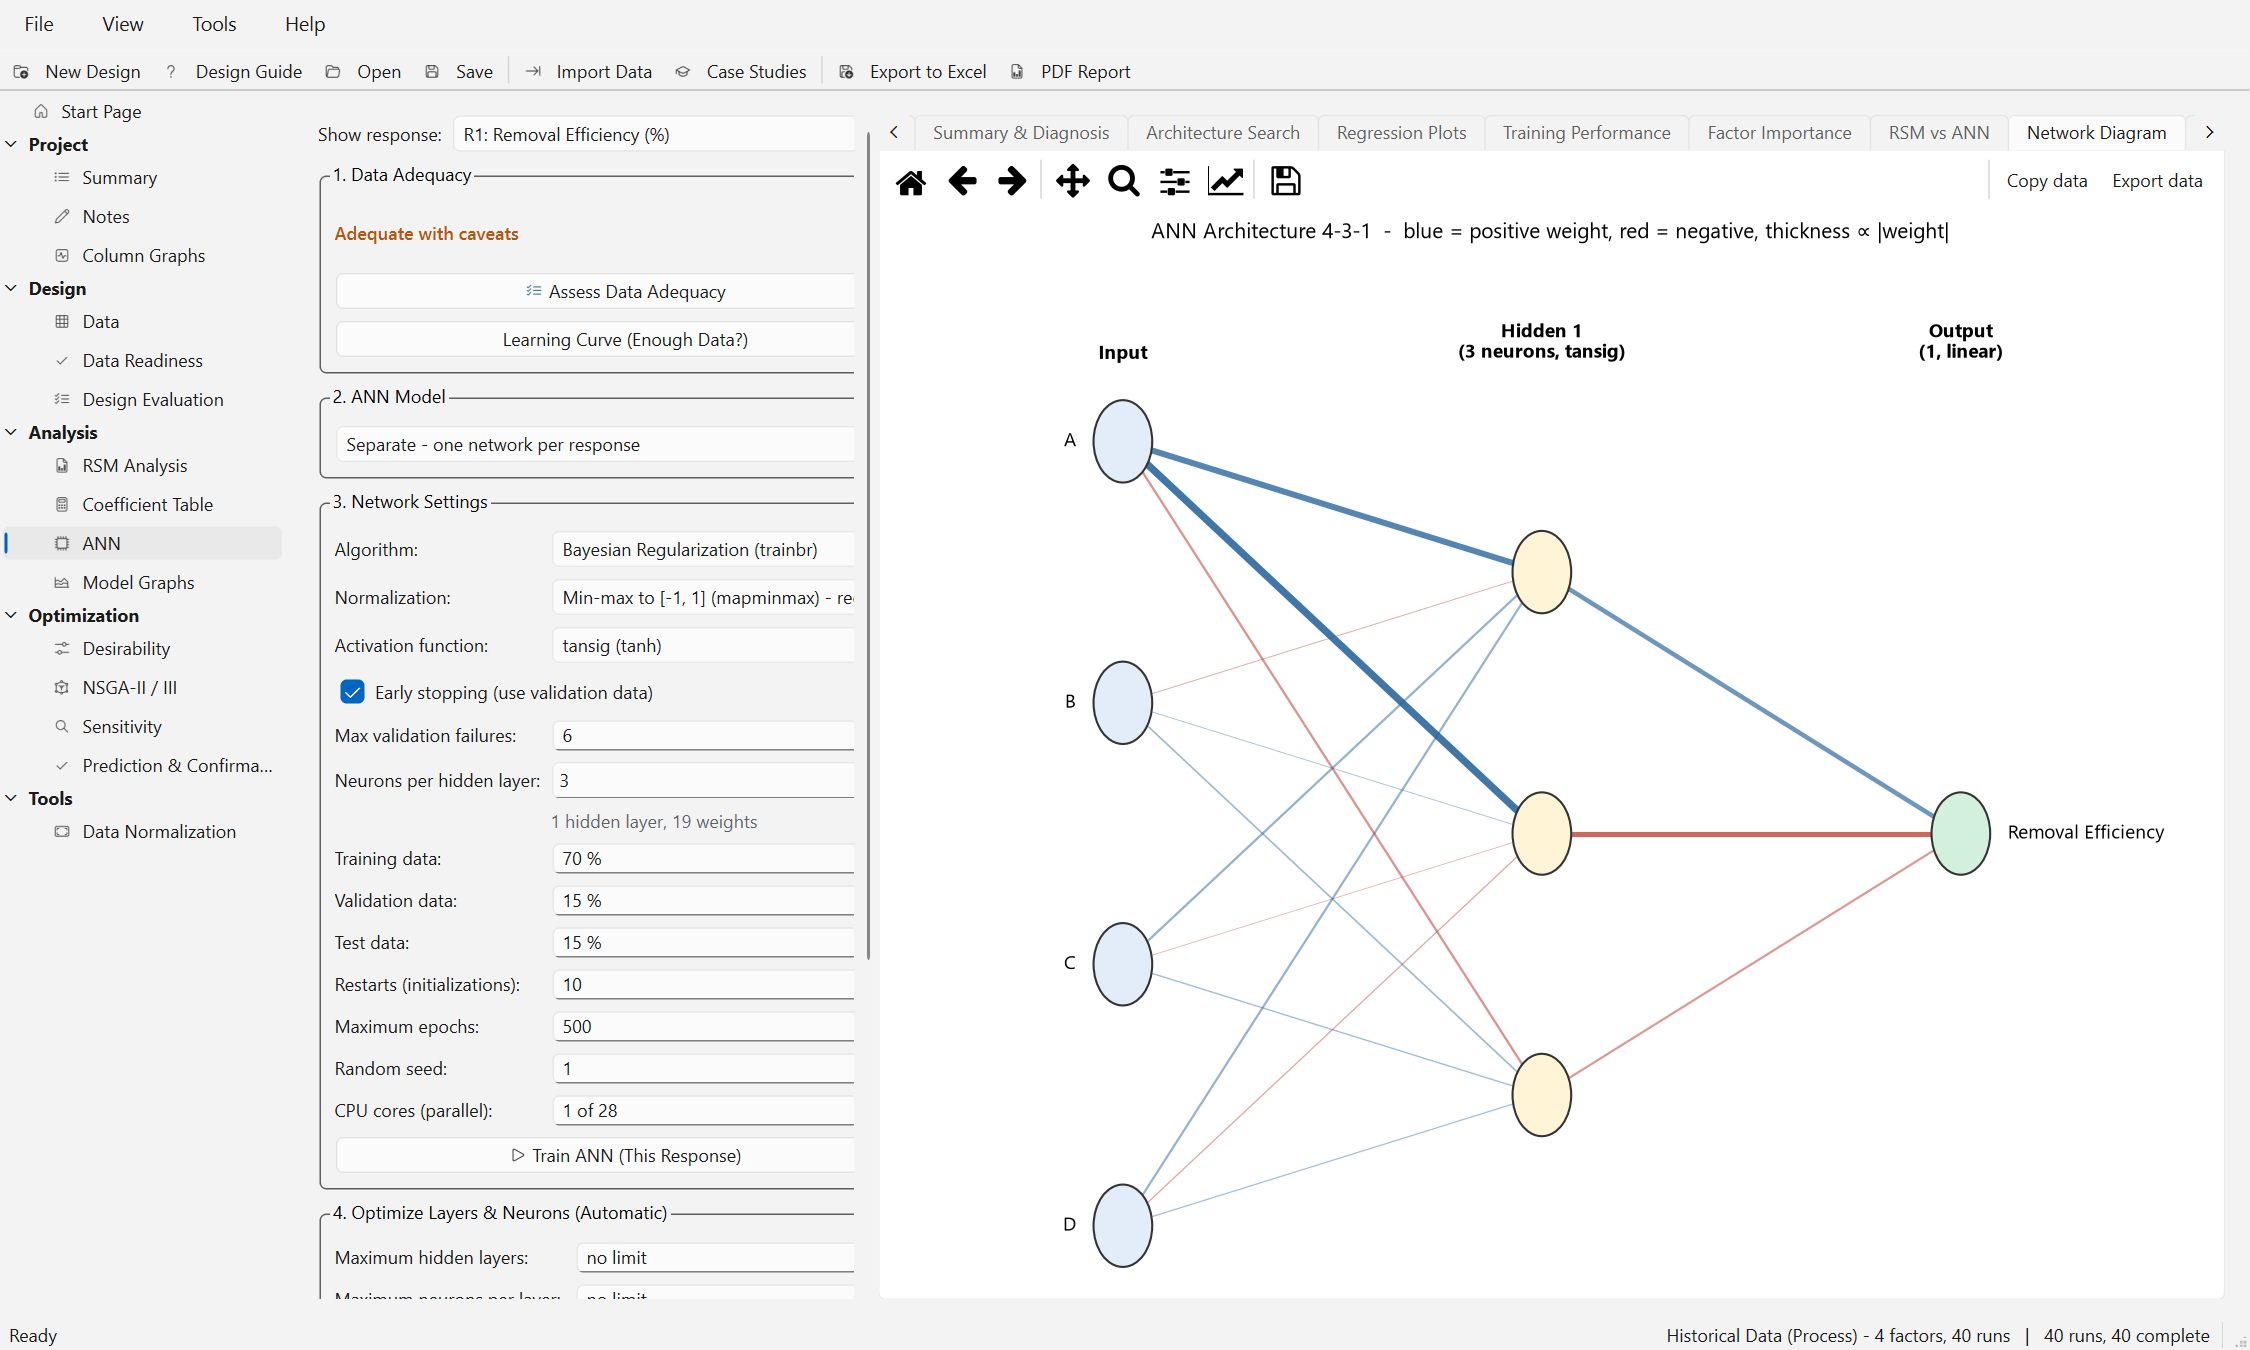
\includegraphics[width=\linewidth]{ann_diagram.png}
\caption{\ui{Network Diagram} of the 4-3-1 network.}
\label{fig:ch07-diagram}
\end{figure}

\paragraph{Weights \& Biases.} Tables of the input-to-hidden weights and biases (IW, b1), the weights between hidden
layers, the hidden-to-output weights and output biases (LW, b output), and the normalization parameters (min and
max of the training and validation runs, offset, scale, base) of every input and output
(Figure~\ref{fig:ch07-weights}). With Eqs.~\eqref{eq:ch07-input}--\eqref{eq:ch07-output} and
\eqref{eq:ch07-normalize} these numbers reproduce the network outside REGEN: code the factors, normalize them,
apply each layer, and convert the output back to response units. The note below the tables states this recipe.

\begin{figure}[htbp]
\centering
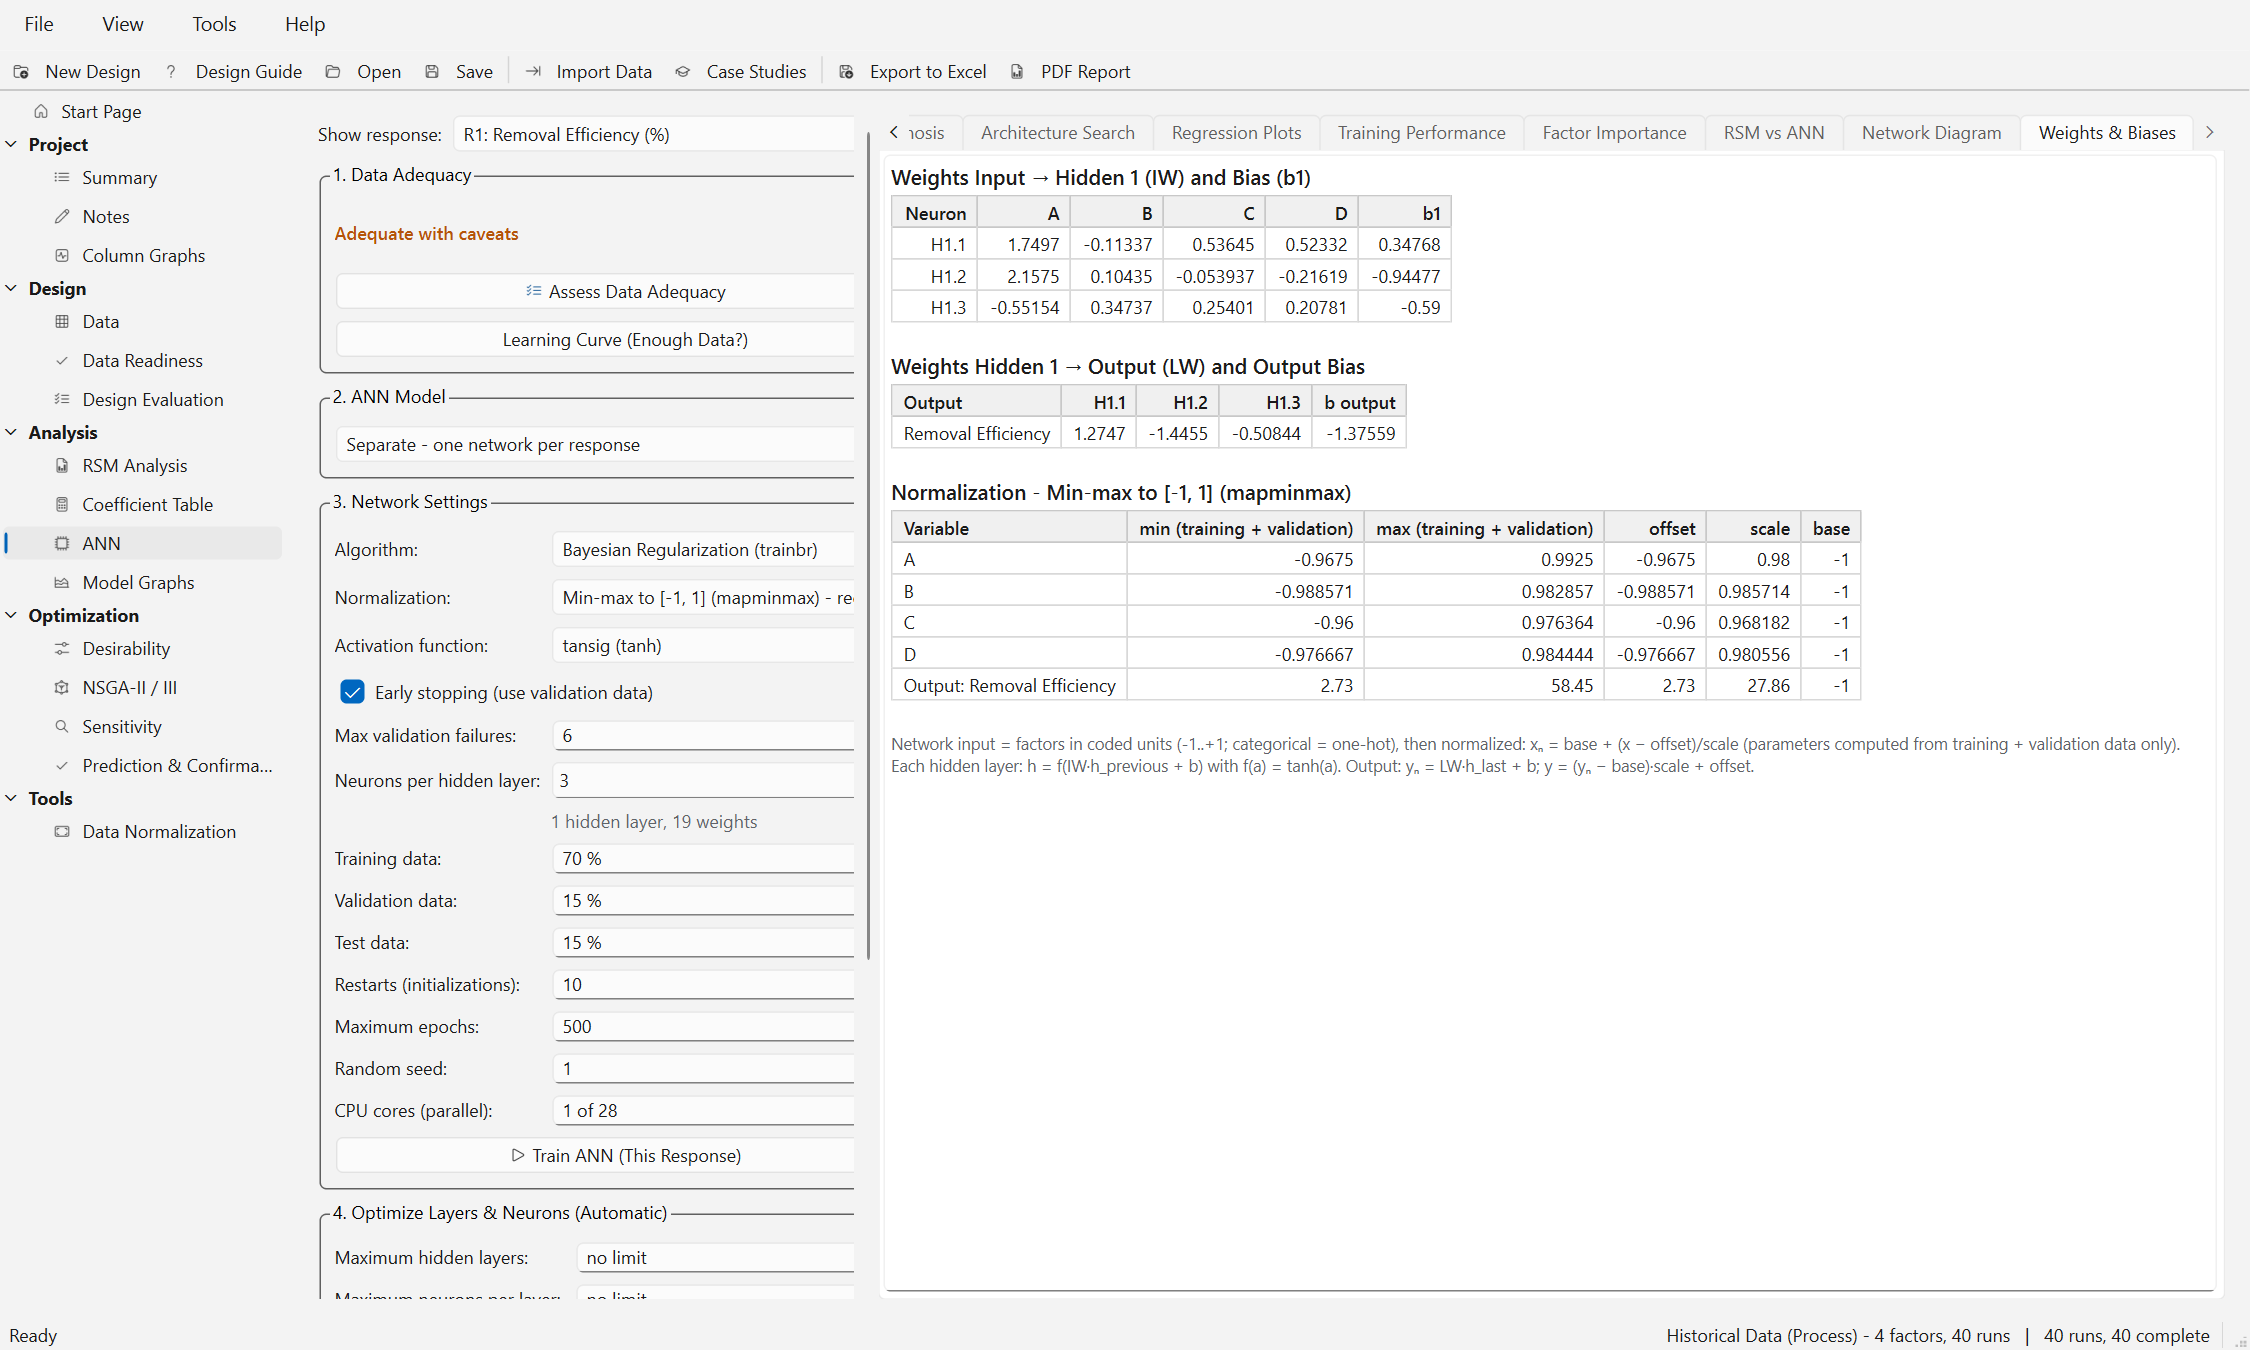
\includegraphics[width=\linewidth]{ann_weights.png}
\caption{\ui{Weights \& Biases} of the 4-3-1 network with the normalization parameters.}
\label{fig:ch07-weights}
\end{figure}

\paragraph{Data export.} Every plot of the page has \ui{Copy data} and \ui{Export data\dots} in its toolbar
(\ui{Copy plot data} and \ui{Export plot data\dots} on right-click); the data behind each panel go to the clipboard,
an Excel workbook or a CSV file. The report tabs (\ui{Data Adequacy}, \ui{Learning Curve}, \ui{Summary \&
Diagnosis}, \ui{Architecture Search}, \ui{Weights \& Biases}) offer \ui{Export all tables\dots} on right-click,
which writes each table to its own sheet.

\section{Using the network in other pages}\label{sec:ch07-use}

The check box \ui{Use this response's ANN for graphs, optimization, NSGA-II \& prediction} is available once the
shown response has a network. When it is ticked, the network replaces the RSM model of that response on the
\ui{Model Graphs}, \ui{Desirability}, \ui{NSGA-II / III}, \ui{Sensitivity} and \ui{Prediction \& Confirmation}
pages. The same choice is made per response in the \ui{Model} column of the desirability and NSGA tables. A network
gives point predictions only: confidence and prediction intervals are not available (Chapter~\ref{chap:10}), and the
confirmation rule for an ANN is a tolerance on the error.

Select the ANN only when it predicts new data better than RSM, judged by the cross-validated test $R^2$ of the
search against the RSM test $R^2$ on the same folds and the RSM Predicted $R^2$. When an optimization depends on
the choice of model, the comparison of the RSM and ANN Pareto fronts (check~D, Chapter~\ref{chap:8}) shows how much, and
confirmation runs settle the question.

\section{Parallel processing}\label{sec:ch07-parallel}

Training many networks is the slowest part of REGEN. \ui{CPU cores (parallel):} sets the number of processor cores
used (default: all logical cores but one, so the computer stays responsive). The work is divided into independent
jobs:
\begin{itemize}
  \item in the architecture search, every combination of candidate network, data split and restart is one job.
    When there are more cores than jobs per candidate, the next few neuron counts (at most patience $+2$) are
    evaluated together; they are recorded in order and candidates after a stop are discarded, so the decisions are
    the same as on one core;
  \item in the learning curve, every point of every repeat is one job;
  \item in \ui{Train ANN}, the restarts run in parallel when the work is large enough to pay for starting the
    worker processes (estimated as training runs $\times$ weights $\times$ outputs $\times$ epochs $\times$
    restarts $\ge 3\times10^7$) or when the workers are already running;
  \item \ui{Optimize All Responses (One Click)} searches several responses at the same time when at least 16 cores
    are selected (one response per 8 cores).
\end{itemize}
Each job has its own random generator derived from the seed, so the results do not depend on the number of
cores; only the time does. The worker processes use one thread each and are closed after 90~s without work. The
work runs in the background so the window stays responsive; \ui{Stop} cancels it (the status line shows
``Stopping\dots''). For data sets with more than 5000 runs, the final training uses at most $\max(3,
\text{cores})$ restarts (``large data (\dots{} runs): restarts limited to \dots''). If a worker process fails, for
example for lack of memory, the message is ``A parallel process stopped unexpectedly (possibly not enough
memory).''; reduce the number of cores or the network size.

\section{Saving results}\label{sec:ch07-saving}

\menupath{File $\rightarrow$ Save} stores in the project file every trained network (weights, normalization, data
split, settings, training history, single-split and cross-validated diagnosis), the choice between RSM and ANN for
each response, the architecture search results and the learning curves. When the project is opened again, the
tabs show the saved results without retraining; the data adequacy report is recomputed. A search result larger
than about 5 million characters (very large searches) is not saved; the network itself is always saved. Changing
the data after a search does not update the saved results: repeat the search and the learning curve after adding
or excluding runs.

\section{Practical advice and limitations}\label{sec:ch07-advice}

\begin{itemize}
  \item An ANN is a data-hungry model. With fewer than about 20--30 runs, a well-chosen RSM model is usually more
    reliable, and the search will often show that RSM predicts new data as well as the ANN. Designed experiments
    with few runs (a Box-Behnken design with 17 runs) rarely support an ANN.
  \item Always judge an ANN by data it has not seen: the cross-validated test $R^2$ of the search, the learning
    curve, and finally confirmation runs (Chapter~\ref{chap:10}). Training $R^2$ alone says nothing about prediction.
  \item The random seed changes the data split and the initial weights. With small data sets, results can change
    noticeably with the seed; this is another reason to rely on cross-validation.
  \item An ANN extrapolates poorly. Predictions outside the region covered by the runs (including gaps inside it)
    can be far off even when the test $R^2$ is high.
  \item The network has no confidence or prediction intervals in REGEN. Its uncertainty is summarized only by the
    cross-validated test RMSE.
  \item The noise rules of the diagnosis need replicated runs. Without them, overfitting can only be detected from
    the error on new data.
\end{itemize}
